\documentclass{deltares_manual}

\usepackage{tikz}
\usepackage[pipeTables=true]{markdown}

%------------------------------------------------------------------------------
\newcommand{\dfastbe}{\textrm{D-FAST~Bank~Erosion}\xspace}

\hypersetup
{
    pdfauthor   = {Deltares},
    pdftitle    = {\dfastbe},
    pdfkeywords = {Deltares User Manual \dfastbe}
}

%------------------------------------------------------------------------------
%

%\makeindex

%------------------------------------------------------------------------------
%
\begin{document}
\pagestyle{empty}
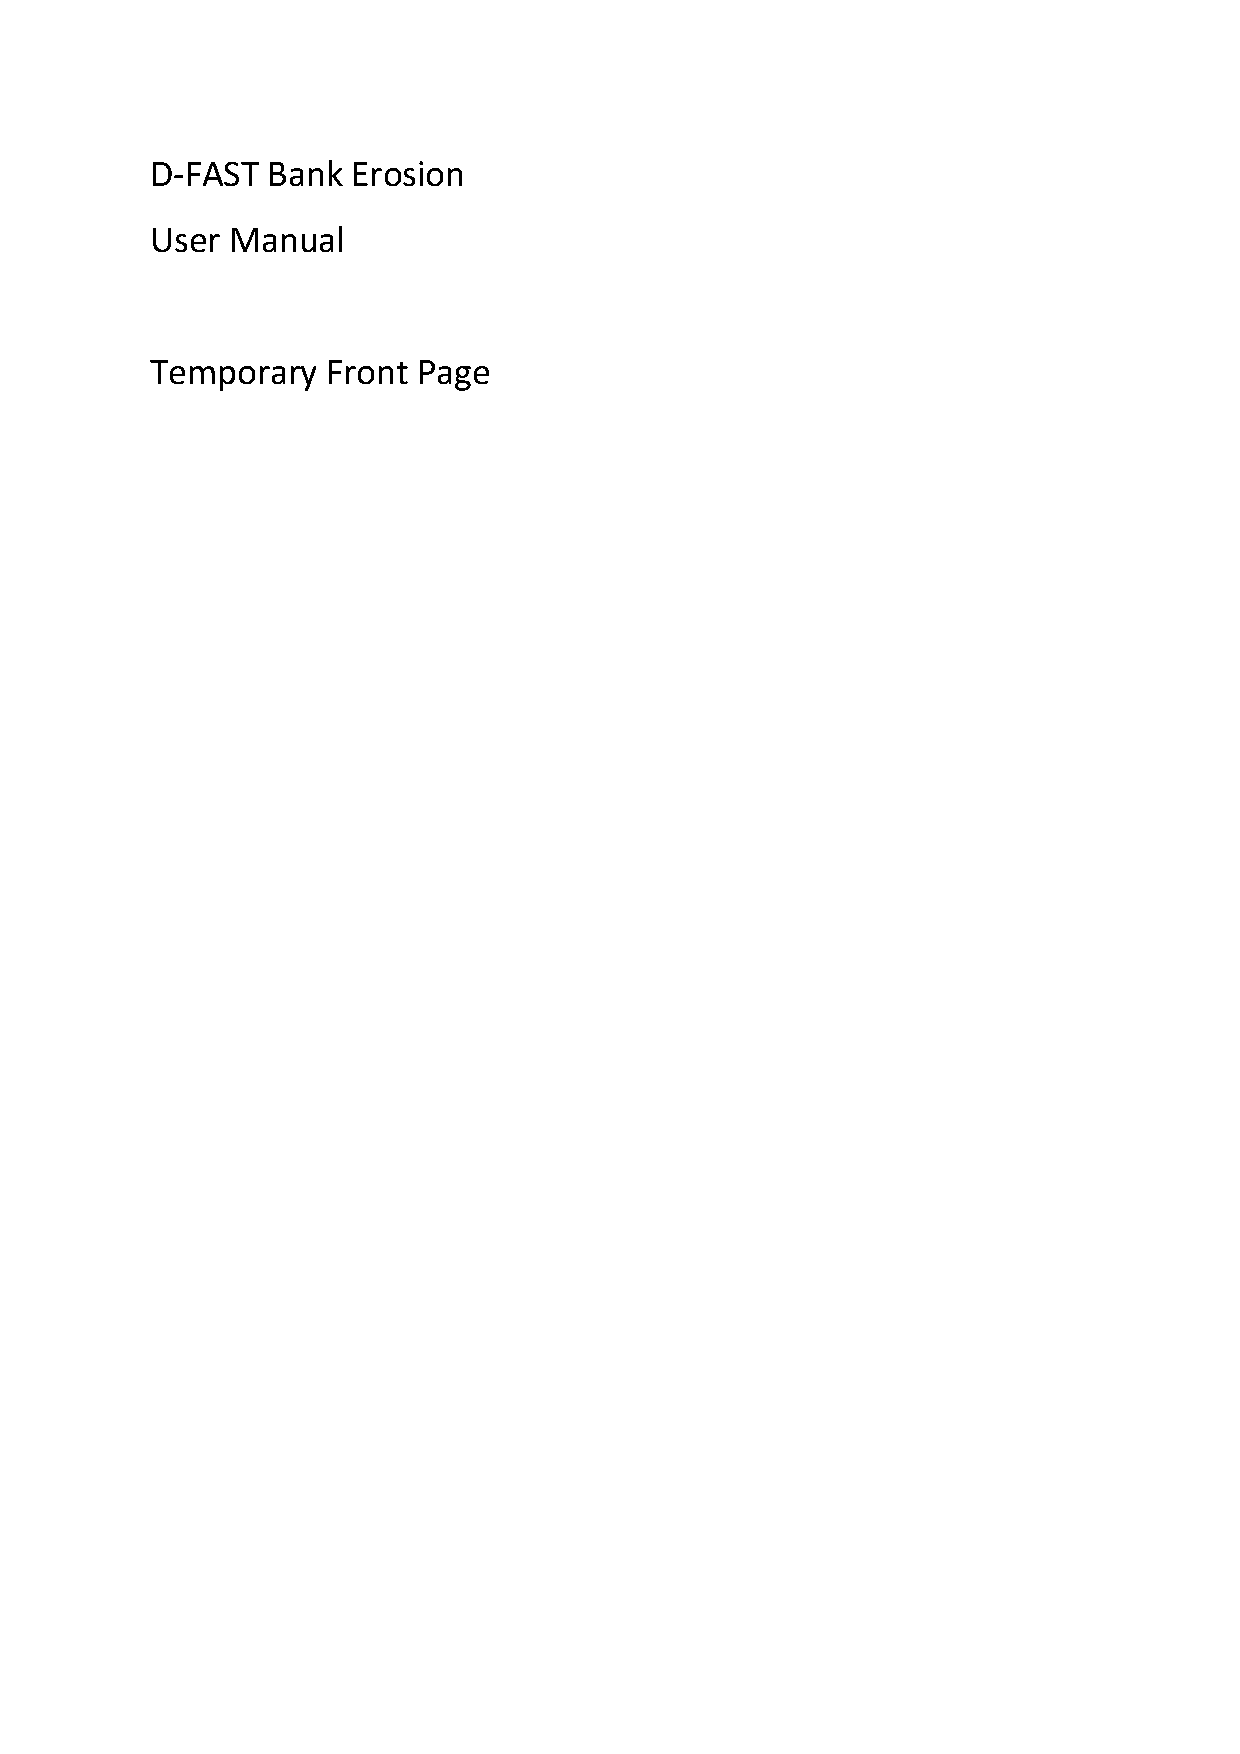
\includepdf[pages=1, offset=72 -70]{cover/d-fast-bank-erosion.pdf} % links-rechts past precies
\cleardoublepage
\title{\dfastbe}
\subtitle{}
\manualtype{User Manual}
\version{0.1}

\author{ }

\deltarestitle
%
\chapter{Introduction}

Since 2010 Deltares is working on a bank erosion module that can be used in combination with D-Flow FM.
The module computes local erosion sensitivity, visualizes the bank movement and gives an estimation of the amount of bank material that is released in the first year and after the equilibrium is reached.
\dfastbe can easily be used as a post processing tool of D-Flow FM-simulations.
Some examples for which \dfastbe can compute bank erosion are:

\begin{itemize}
\item Bank adjustments such as removal of bank protection
\item Applying or removing fore shore protection
\item Changes in shipping type or intensity
\item Changes in currents (e.g. due to construction of side channels)
\end{itemize}

\subsubsection*{Output}
The output of \dfastbe is:

\begin{enumerate}
\item Bank line movement after one year and when the final equilibrium state is reached.
\item Amount of sediment that is released from the banks after one year and when the final equilibrium state is reached.
\end{enumerate}

This output is presented in graphs / figures and written to text files.

\subsubsection*{Input}
The input of \dfastbe is:

\begin{enumerate}
\item D-Flow FM results (NetCDF map-files)
\item Local data: level of bank protection removal, subsoil characteristics, shipping information (quantity, location of fairway)
\end{enumerate}

The layout of this manual is as follows: In this chapter a description is given on how to use \dfastbe (installation, input, output).
The background of \dfastbe is outlined in \autoref{Chp3} and \autoref{Chp4} (partly in Dutch).

\section{Installation}

\dfastbe itself consists of 2 executables called 'BankLines.exe' and BankErosion.exe'.
The first is needed to establish the initial bank lines and the second computes the bank line movement and eroded volume.
Both executables of \dfastbe can be called from the DOS prompt.

To be able to run \dfastbe it is necessary to install MCRinstaller.
The required version of the installer is standard provided with \dfastbe.

By default \dfastbe is looking for the definition file deffile.def in the same directory as the executables.
When the definition file has another name or location, this should be passed when the modules are called.

\section{Scenario plan}

\dfastbe is not calibrated for local bank erosion\footnote{This is almost impossible, due to other uncertainties in bank properties, limited availability of field data of measured bank erosion and the fact that WAQUA computes longer river reaches.
Locally \dfastbe could be calibrated when historical data of bank erosion is available.
However, this does not automatically imply that a few kilometers downstream \dfastbe gives good results with the same settings, because the bank properties can be completely different.}.
Therefore it is strongly advised to use \dfastbe only in a \emph{relative} way.
In this way an image can be formed of

\begin{itemize}
\item at which locations the bank is most sensitive to erosion (by comparing different locations along the river)
\item how sensitive a location is for certain measures (by comparing different scenarios at 1 location)
\end{itemize}

We advise to compute different scenarios and compare between them.
An example is: 1 scenario with a subsoil of sand and 1 scenario with a subsoil of clay.
This means that only the type of subsoil is changed and the other input remains unchanged.

\section{D-Flow FM-computations}

Before \dfastbe can be used, steady state D-Flow FM-computations\footnote{D-Flow FM-models and Baseline schematisations of the Dutch river system can be applied by Helpdeskwater.nl Onderwerpen > Applicaties en modellen > Water en ruimte > Gebiedsschematisaties > Servicedesk > Meldingsformulier} have to be performed for each discharge level.
This first requires a schematisation of the discharge hydrograph in discharge levels and a probability per discharge step.
The discretisation of the discharge hydrograph is not a trivial procedure.
Deltares advises to use at least ten discharge levels.

By default two figures are generated during \dfastbe computation which the user can use to check if the discharge levels are chosen properly.
These are a figure with water levels and a figure with flow velocities.
In both figures the area that is sensitive to erosion is indicated.
Based on these figures it can be decided to include or remove discharge levels from the computation.
For each discharge level an NetCDF map-file (D-Flow FM output file) must be provided.
\dfastbe uses the water levels and flow velocities that are stored in the last time step.
It is important that the D-Flow FM computations are in steady state.
The probability (normalized weighting of the time period) per discharge level is defined by the user in the definition file.

Note: It is of utmost importance that in the NetCDF map-file with the reference (average) discharge (which is used to establish the initial bank lines) the water remains within the main channel during the whole computation.
Practically this means that the simulation has to be started with a low initial water level with no (or as little as possible) water in the flood plains.
When this criterion is not met, strange peaks in the detected bank lines may occur.



An example of discharge levels for the river Meuse in combination with different probabilities for different scenarios (wet/dry/intermediate) is given in \autoref{Tab2.1}.

\begin{table}
\begin{tabular}{p{2cm}p{2cm}p{2cm}p{2cm}p{2cm}}
Dicharge level nr. & Discharge (m3/s) & 1998-2002 (wet) & 2004-2010 (dry) & 2008-2011 (intermediate) \\ \hline
1 & 75 & 0.2932 & 0.1808 & 0.3110 \\
2 & 150 & 0.1918 & 0.2466 & 0.2329 \\
3 & 272 & 0.1918 & 0.2603 & 0.2055 \\
4 & 400 & 0.0411 & 0.0548 & 0.0685 \\
5 & 500 & 0.1507 & 0.1370 & 0.0959 \\
6 & 750 & 0.0548 & 0.0712 & 0.0548 \\
7 & 900 & 0.0329 & 0.0384 & 0.0164 \\
8 & 1100 & 0.0164 & 0.0082 & 0.0055 \\
9 & 1300 & 0.0137 & 0.0014 & 0.0021 \\
10 & 1500 & 0.0041 & 0.0014 & 0.0021 \\
11 & 1700 & 0.0041 & 0.0000 & 0.0021 \\
12 & 1900 & 0.0041 & 0.0000 & 0.0021 \\
13 & 2300 & 0.0014 & 0.0000 & 0.0014 \\ \hline
\end{tabular}
\caption{Probabilities of a discharge level for different scenarios (De Vries, 2012)}
\label{Tab2.1}
\end{table}

\section{Definitionfile <defile.def>}\label{Sec2.4}

The definition file contains input parameters for the executables 'BankLines' en 'BankErosion'.
De executables search for the file 'defile.def' in the same directory as themselves, unless another file or path name is given.
The possible keywords and their description are given in \autoref{Tab2.2}.
The existence, not the order, of the keywords is of importance.

In the table the following abbreviations are used:
\begin{itemize}
\item[M] mandatory
\item[O] optional
\item[E] expert
\end{itemize}

Filenames can be either given with a single filename, or with their (relative) path and they should contain no spaces.
An example of a definition file is given in \autoref{Fig2.1}.

\begin{table}
\begin{tabular}{lllp{5cm}}
Keyword &  & Value & Description \\ \hline
Path & M & pathname & [REMOVED] Pathname of used m-files (unnecessary when using executables) \\
Nbank & M & integer & Number of bank lines, (standard 2 lines) \\
GridFile  & M & filename & Rgf-file for defining grid coordinates \\
RiverKM & M & filename & Textfile with riverkilometres and correspondig xy-coordinates \\
Boundaries  & O & integers & river chainage of the region of interst;  rkm-start:rkm-end, e.g. 81:100 (default: all) \\
NLim & O & integers & [REMOVED] Range of N-values from SDS-file that is considered (default: all), only used when keyword 'Boundaries' is not available. \\
Mlim & O & integers & [REMOVED] Range of M-values from SDS-file that is considered (default: all), only used when keyword 'Boundaries' is not available. \\
Plotting & O & logical & [REMOVED] Plotting results (default: false) \\
SavePlots & O & Logical & [REMOVED] Saving plots (default: true) \\
ClosePlots & O & Logical & [REMOVED] Close plots and close Quickplot when simulation is finished (default: false) \\
Waqview & O & logical & [REMOVED] Generating output for Waqview (default: false) \\ \hline
\end{tabular}
\caption{Keywords in the definition file of \dfastbe}
\label{Tab2.2}
\end{table}

Input BankLines.exe

\begin{tabular}{lllp{5cm}}
Keyword &  & Value & Description \\ \hline
SDS-file & M & filename & [REPLACE BY File] SDS-file for determining representative bank line \\
Line1    & M & filename & Textfile with xy-coordinates of search line 1 \\
LineN    & M & filename & Textfile with xy-coordinaten of search line N \\
BankDir & O & string & Directory for storing bank lines (default: current directory) \\
BankFile & O & filename & Text file(s) in which xy-coordinates of bank lines are stored (default 'bankfile') \\
LocalDir & O & filename & Directory for storing local output (default: 'local') \\
SortLim & E & real & Maximum number of vertices used for sorting (default: 50) \\
Waterdepth & E & real & Water depth used for defining bank line (default 0.0) \\
Dlines & E & nline reals & Distance from pre-defined lines used for determining bank lines (default: 50) \\
Dremove & E & nline reals & Ommiting coordinates that are more than this distance from neighbouring points (default: 5000) \\ \hline
\end{tabular}

Input BankErosion.exe

\begin{tabular}{lllp{5cm}}
Keyword &  & Value & Description \\ \hline
Terosion & M & real & Simulation period  [years] \\
RiverAxis & M & filename & Textfile with xy-coordinates of river axis \\
Fairway  & M & filename & Textfile with xy-coordinates of fairway axis \\
BankType & M & filename/real & Bank strength definition (for each bank line per river-km) \\
Vship  & M & filename/real & Relative velocity of the ships (per river-km) [m/s] \\
Nship  & M & filename/integer & Number of ships per year (per river-km) \\
ShipType & M & filename/integer & Type of ship (per river-km) \\
Draught & M & filename/real & Draught of the ships (per river-km) [m] \\
NLevel & M & integer & Number of discharge levels \\
File1 & M & filename & [REPLACES SDSfile1] NetCDF map-file for computing bank erosion for discharge 1 (only used when 'Nlevel'>1) \\
PDischarge1 & M & real & Probability of discharge 1 (sum of probabilities should be 1) \\
FileN & M & filename & [REPLACES SDSfileN] NetCDF map-file for computing bank erosion for discharge 'Nlevel' (only used when 'Nlevel'>1) \\
PDischargeN & M & real & Probability of discharge 'Nlevel' (sum of probabilities should be 1) \\
RefLevel & O & integer & Reference level: discharge level with SDS-file that is equal to 'SDS-file' (only used when 'Nlevel'>1)  (default: 1) \\
Classes & O & logical & Use classes (true) or critical shear stress (false) in 'BankType' (default: true) \\
ProtectLevel & O & filename & Text file(s) with level of bank protection for each bank line per river-km (default: -1000) \\
Slope & O & filename & Text file(s) with equilibrium slope for each bank line per river-km  (default: 20) \\
OutputDir & O & String & Directory for storing output files \\
BankNew & O & filename & Text file(s) in which new xy-coordinates of bank lines are stored (default 'banknew') \\
BankEq & O & filename & Text file(s) in which xy-coordinates of equilibrium bank lines are stored (default: 'bankeq') \\
EroVol & O & filename & Text file in which eroded volume per river-km is stored (default: 'erovol.evo') \\
OutputInterval & O & real & interval in which the output (eroded volume) is given (default: 1 km) [km] \\
VelFilter & E & logical & Filtering velocity along bank lines (default: true) \\
Revert & E & nline integers & Reverting direction of erosion (default 0) \\
Wave0 & E & real & Distance from fairway axis at which waveheight is zero (default 200 m) \\
Wave1 & E & real & Distance from fairway axis at which reduction of waveheigth to zero starts (default Wave0-50 m) \\
Nwave & E & integer & Number of waves per ship (default 5) \\ \hline
\end{tabular}

\begin{figure}
\begin{verbatim}
    % General input parameters bank erosion module
    NBank          = 2
    GridFile       = inputfiles\maas40m_1.rgf
    RiverKM        = inputfiles\rivkm.xyc
    Boundaries     = 123:128
    WaqView        = true
    Plotting       = true
    %
    % Input parameters bank line detection
    Bankdir        = output\banklines
    SDSfile        = inputfiles\SDS-q272
    Line1          = inputfiles\oeverlijn_links_mod.xyc
    Line2          = inputfiles\oeverlijn_rechts_mod.xyc
    %
    % Input parameters bank erosion module
    OutputDir      = output\bankerosion
    Terosion       = 1
    RiverAxis      = inputfiles\maas_rivieras_mod.xyc
    Fairway        = inputfiles\maas_rivieras_mod.xyc
    Classes        = false
    BankType       = inputfiles\bankstrength_tauc
    Vship          = 5.0
    Nship          = inputfiles\nships_total
    ShipType       = 2
    Draught        = 2.5
    ProtectLevel   = inputfiles\stortsteen
    Slope          = inputfiles\slope
    BankEq         = bankequi
    EroVol         = erovol_standard.evo
    OutputInterval = 0.1
    Revert         = [1,0]
    %
    % Discharge dependent parameters
    NLevel         = 10
    RefLevel       = 3
    SDSfile1       = SDSfiles\SDS-q75
    PDischarge1    =   0.1808
    SDSfile2       = SDSfiles\SDS-q150
    PDischarge2    =   0.2466
    SDSfile3       = SDSfiles\SDS-q272
    PDischarge3    =   0.2603
    SDSfile4       = SDSfiles\SDS-q400
    PDischarge4    =   0.0548
    SDSfile5       = SDSfiles\SDS-q500
    PDischarge5    =   0.1370
    SDSfile6       = SDSfiles\SDS-q750
    PDischarge6    =   0.0712
    SDSfile7       = SDSfiles\SDS-q900
    PDischarge7    =   0.0384
    SDSfile8       = SDSfiles\SDS-q1100
    PDischarge8    =   0.0082
    SDSfile9       = SDSfiles\SDS-q1300
    PDischarge9    =   0.0014
    SDSfile10      = SDSfiles\SDS-q1500
    PDischarge10   =   0.0014
\end{verbatim}
\caption{Example of a definition file for \dfastbe}
\label{Fig2.1}
\end{figure}

\section{Banklines <BankLines.exe>}

determines the representative bank lines within the area of interest (for background information see chapter 3).
The input of Banklines is given through the definition file (deffile.def), see \autoref{Sec2.4}.

When the definition file has the name deffile.def and is located in the same directory as the executable the module can be called as follows:

\begin{Verbatim}
BankLines
\end{Verbatim}

If the definition file has another name and/or is located in another directory the following call should be used:

\begin{Verbatim}
BankLines path\\deffile\_other.txt
\end{Verbatim}

with \command{path} the path to the directory where the definition file is located and \command{deffile\_other.txt} the name of the definition file.

Required input:

\begin{itemize}
\item D-Flow FM-output file (NetCDF map-file) at representative discharge (\command{SDSfile}),
\item Number of bank Lines (\command{Nbank} default two, the left and right bank),
\item For each of the bank lines a file with xy-coordinates of the estimated location of the bank line (\command{Line1}, \command{Line2}, ..., \command{LineN}, with N the number of bank lines)
\item File which links river kilometres to xy-coordinates (\command{RiverKM}),
\end{itemize}


Optional

\begin{itemize}
\item Area of interest in the form of a range of river kilometres or in terms of mn-coordinates (\command{Boundaries} or \command{NLim} and \command{MLim}).
\item Name of the directory to which the output will be written (\command{BankDir})
\end{itemize}

Output:

\begin{itemize}
\item XY-coordinates of the determined bank lines.
\item Plot of the bank lines (optional, \command{Plotting})
\end{itemize}

The computation has ended successfully when the message "BankLines ended successfully!" appears.

An example of the output as is generated with Banklines.exe is shown in \autoref{Fig2.2}.
The water depth is given with colored surfaces (per grid cell), the black lines are the determined bank lines and the river kilometers are displayed on the river axis.

Note: To obtain the best results, the points of the estimated location of the banks given in  \command{Line1}, \command{Line2}, ..., \command{LineN} (obtained for example from the 'oeverlijnen' from Baseline data), should be equally distributed along the bank with a distance that is in the same order of the gridcellsize along the bank.
Large distances between the points will result in inaccurate bank lines.
Adding points inbetween the points will resolve this problem.
Points too close to eachother will result in large computation times, which can be solved by removing unnecessary points.

\begin{figure}
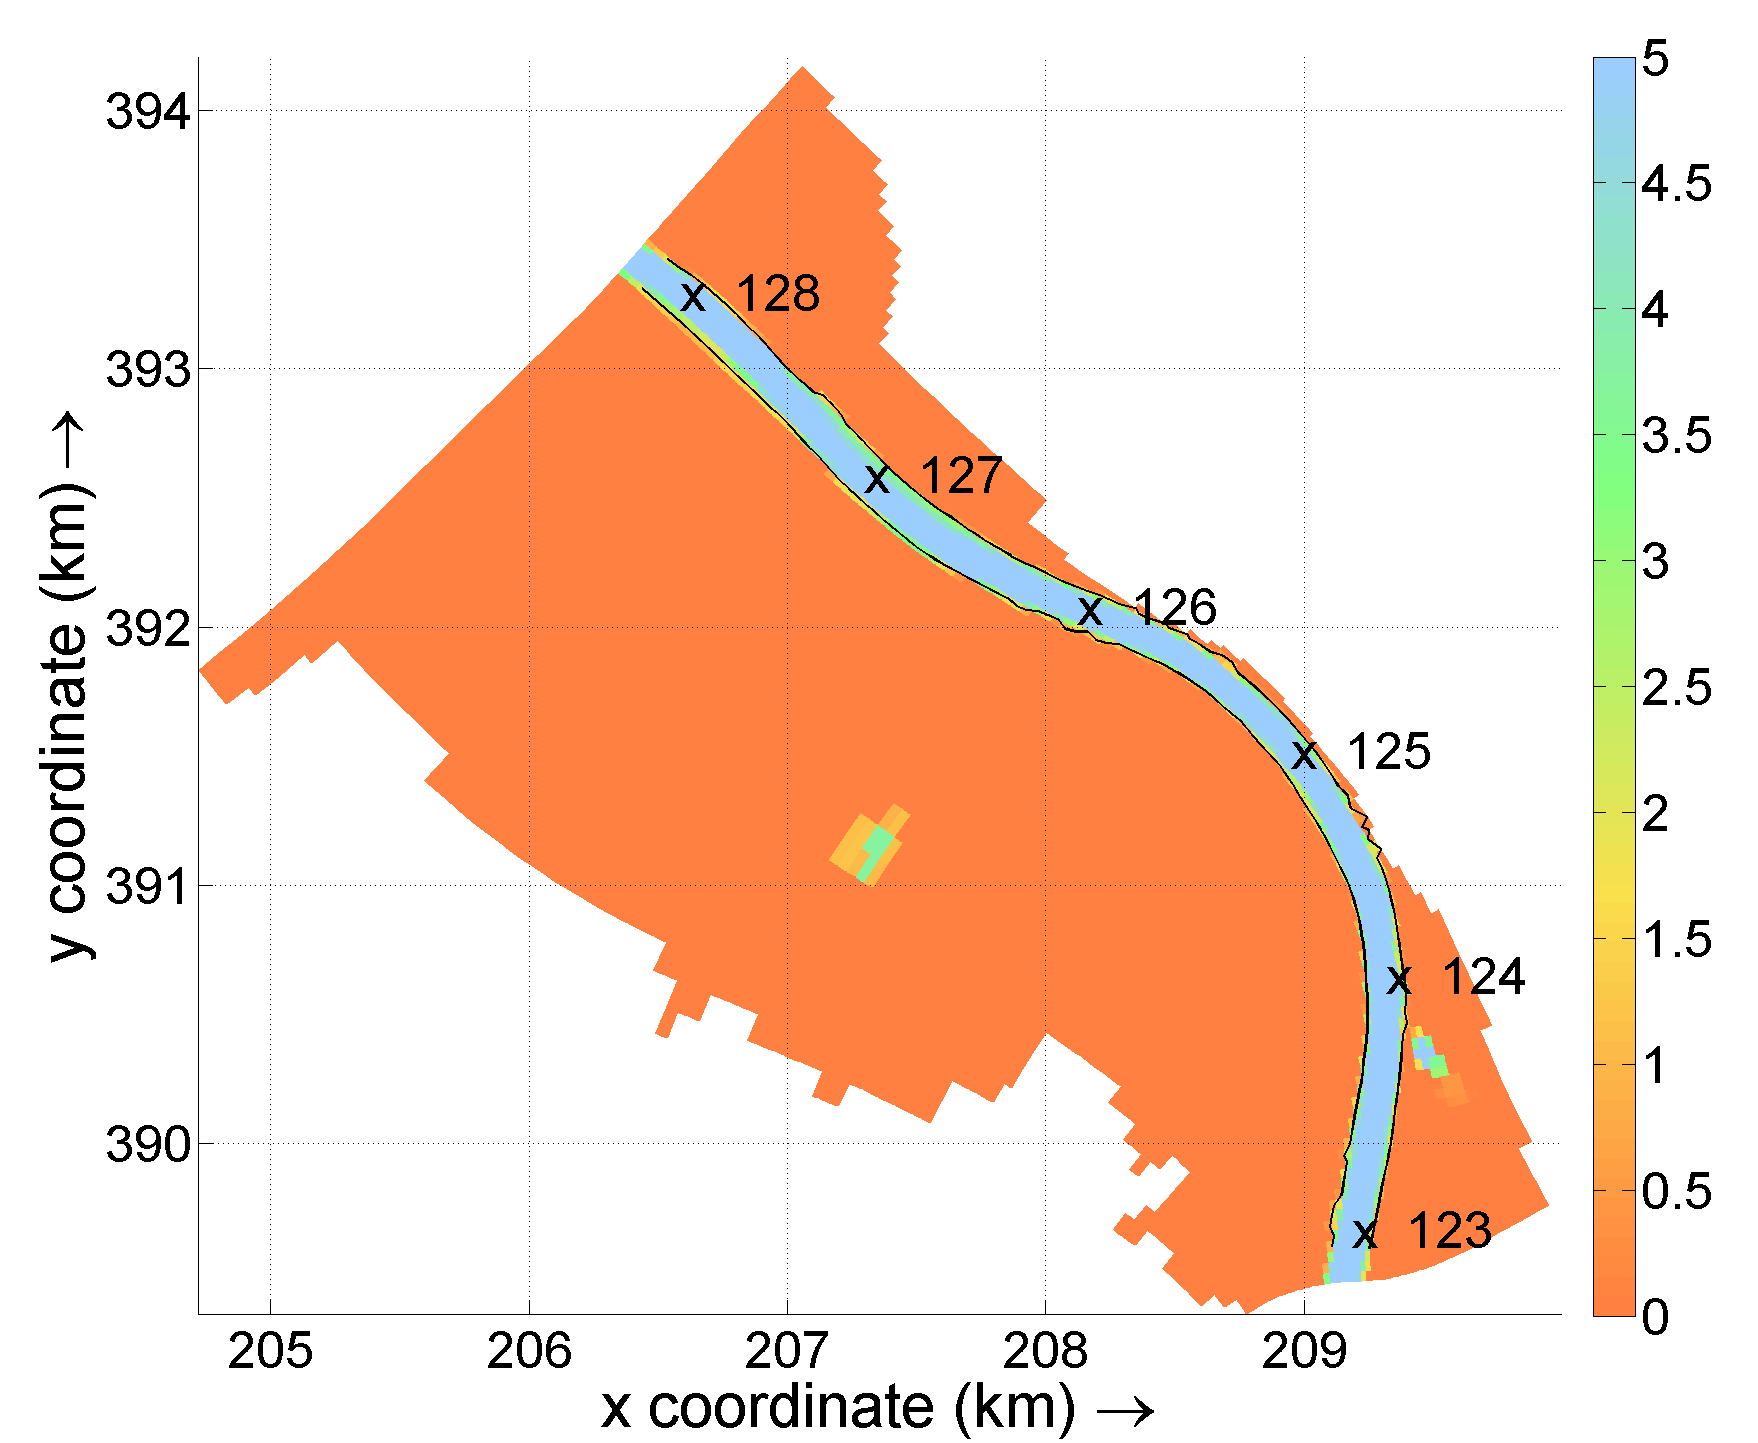
\includegraphics[width=\textwidth]{figures/Fig2-2.png}
\caption{Example of output of BankLines.exe}
\label{Fig2.2}
\end{figure}

\section{BankErosion <BankErosion.exe>}

determines the expected bank erosion within the area of interest (for background information see chapter 4).
The input of BankErosion  is given through the definition file (deffile.def), see \autoref{Sec2.4}.

When the definition file has the name deffile.def and is located in the same directory as the executable the module can be called as follows:

\begin{Verbatim}
BankErosion
\end{Verbatim}

If the definition file has another name and/or is located in another directory the following call should be used:

\begin{Verbatim}
BankErosion path\\deffile\_other.txt
\end{Verbatim}

with \command{path} the path to the directory where the definition file is located and \command{deffile\_other.txt} the name of the definition file.

A clean start can be made with the command:

\begin{Verbatim}
BankErosion deffile.def clean
\end{Verbatim}

This assures that all local files (in the directory \command{LocalDir}), which are specific for a certain reach and discharge levels, are removed.
At the next call of BankLines they are created once again.
The creation of these files can be time consuming, so it is recommended not to clean the files when the reach and/or used SDS-files are not changed.

Required input:

\begin{itemize}
\item The considered simulation time (\command{Terosion}, default 1 year),
\item The number of discharge levels (\command{NLevel}),
\item D-Flow FM-output files (NetCDF map-files) for the different discharge levels and the corresponding probability distribution (\command{File1, File2, ..., FileN} and \command{PDischarge1, PDischarge2, ..., PDischargeN}, with N the number of discharge levels).
When only 1 discharge level is given, the standard NetCDF map-file (\command{SDSfile}) is used,
\item Grid for positioning of results (\command{GridFile}), only needed when \command{WaqView=true},
\item Number of bank Lines (\command{Nbank} default two, the left and right bank),
\item File which links river kilometres to xy-coordinates (\command{RiverKM}),
\item XY-coordinates of the river and fairway axis (\command{RiverAxis}, \command{Fairway}),
\item Information about the strength or type of the soil of the banks (\command{BankType}).
This can be done either in the form of classes (see Tabel 4.1 for values and explanation) or with a critical shear stress (see \autoref{Tab5.1} for examples).
In the first case \command{Classes=true} should be set and in the second case \command{Classes=false} (default).
The bank strength information can be given either with a fixed value for the whole track or in a ASCII-file per river kilometer (first column river-km, second column bank type, see \autoref{Fig2.3}),
\item Shipping information (\command{Vship}, \command{Nship}, \command{ShipType}, \command{Draught}).
This can be done either with a fixed value for the whole track or in a file per river kilometer (first column river-km, second column shipping information: similar to entering bank type, see \autoref{Fig2.3}).
\end{itemize}

Optional
\begin{itemize}
\item ASCII-file with level of bank protection (wrt NAP) for each bank line per river-km.
(First column river-km, second column bank protection level: similar to entering bank type, see \autoref{Fig2.3}).
By default the bank protection level is 1 meter below the water level of the representative discharge,
\item ASCII-file with slope of foreshore (1:n) for each bank line per river-km.
(First column river-km, second column slope parameter n: similar to entering bank type, see \autoref{Fig2.3}).
Default a slope of 1:20 will be used,
\item Name of the directory to which the output will be written (\command{OutputDir}),
\item Name of the file to which the results will be written (\command{BankNew}, \command{BankEq}, \command{EroVol}),
\item Name of the directory to which local files will be written (\command{LocalDir}).
\end{itemize}

Output:

\begin{itemize}
\item Map with waterdepth, initial bank lines, river kilometers and fairway axis (see \autoref{Fig2.4}),
\item Map with erosion sensitivity of the banks based on computed bank retreat (see \autoref{Fig2.5}),
\item The computed erosion volume during the simulation period split up for left and right bank and for each discharge level (see \autoref{Fig2.6}),
\item Total erosion volume based on equilibrium bank line (see \autoref{Fig2.7}),
\item Control figures for water levels of each discharge (see \autoref{Fig2.8} and \autoref{Fig2.9}),
\item Control figures for flow velocity of each discharge (see \autoref{Fig2.10} and \autoref{Fig2.11}),
\item Map with indication of applied bank type (see \autoref{Fig2.12}),
\item Bank retreat at the end of the simulation period and for the equilibrium situation (see \autoref{Fig2.13}),
\item XY-coordinates of the computed bank lines at the end of the simulation period and of the equilibrium bank lines,
\item Files to be able to visualize information in Waqview.
\end{itemize}

The computation has ended successfully when the message "BankErosion ended successfully!" appears.

\begin{figure}
\begin{Verbatim}
  0.0          1
  75.2         3
  90.3         2
  110.0        0
  130.5        4
  153.1        3
  206.9        2
\end{Verbatim}
\caption{Example of input file for bank strength classes per river kilometer: from 0.0 - 75.2 km class 1, from 75.2 - 90.3 km class 3, etc.
When no information is available, the closest value will be used.}
\label{Fig2.3}
\end{figure}

\begin{figure}
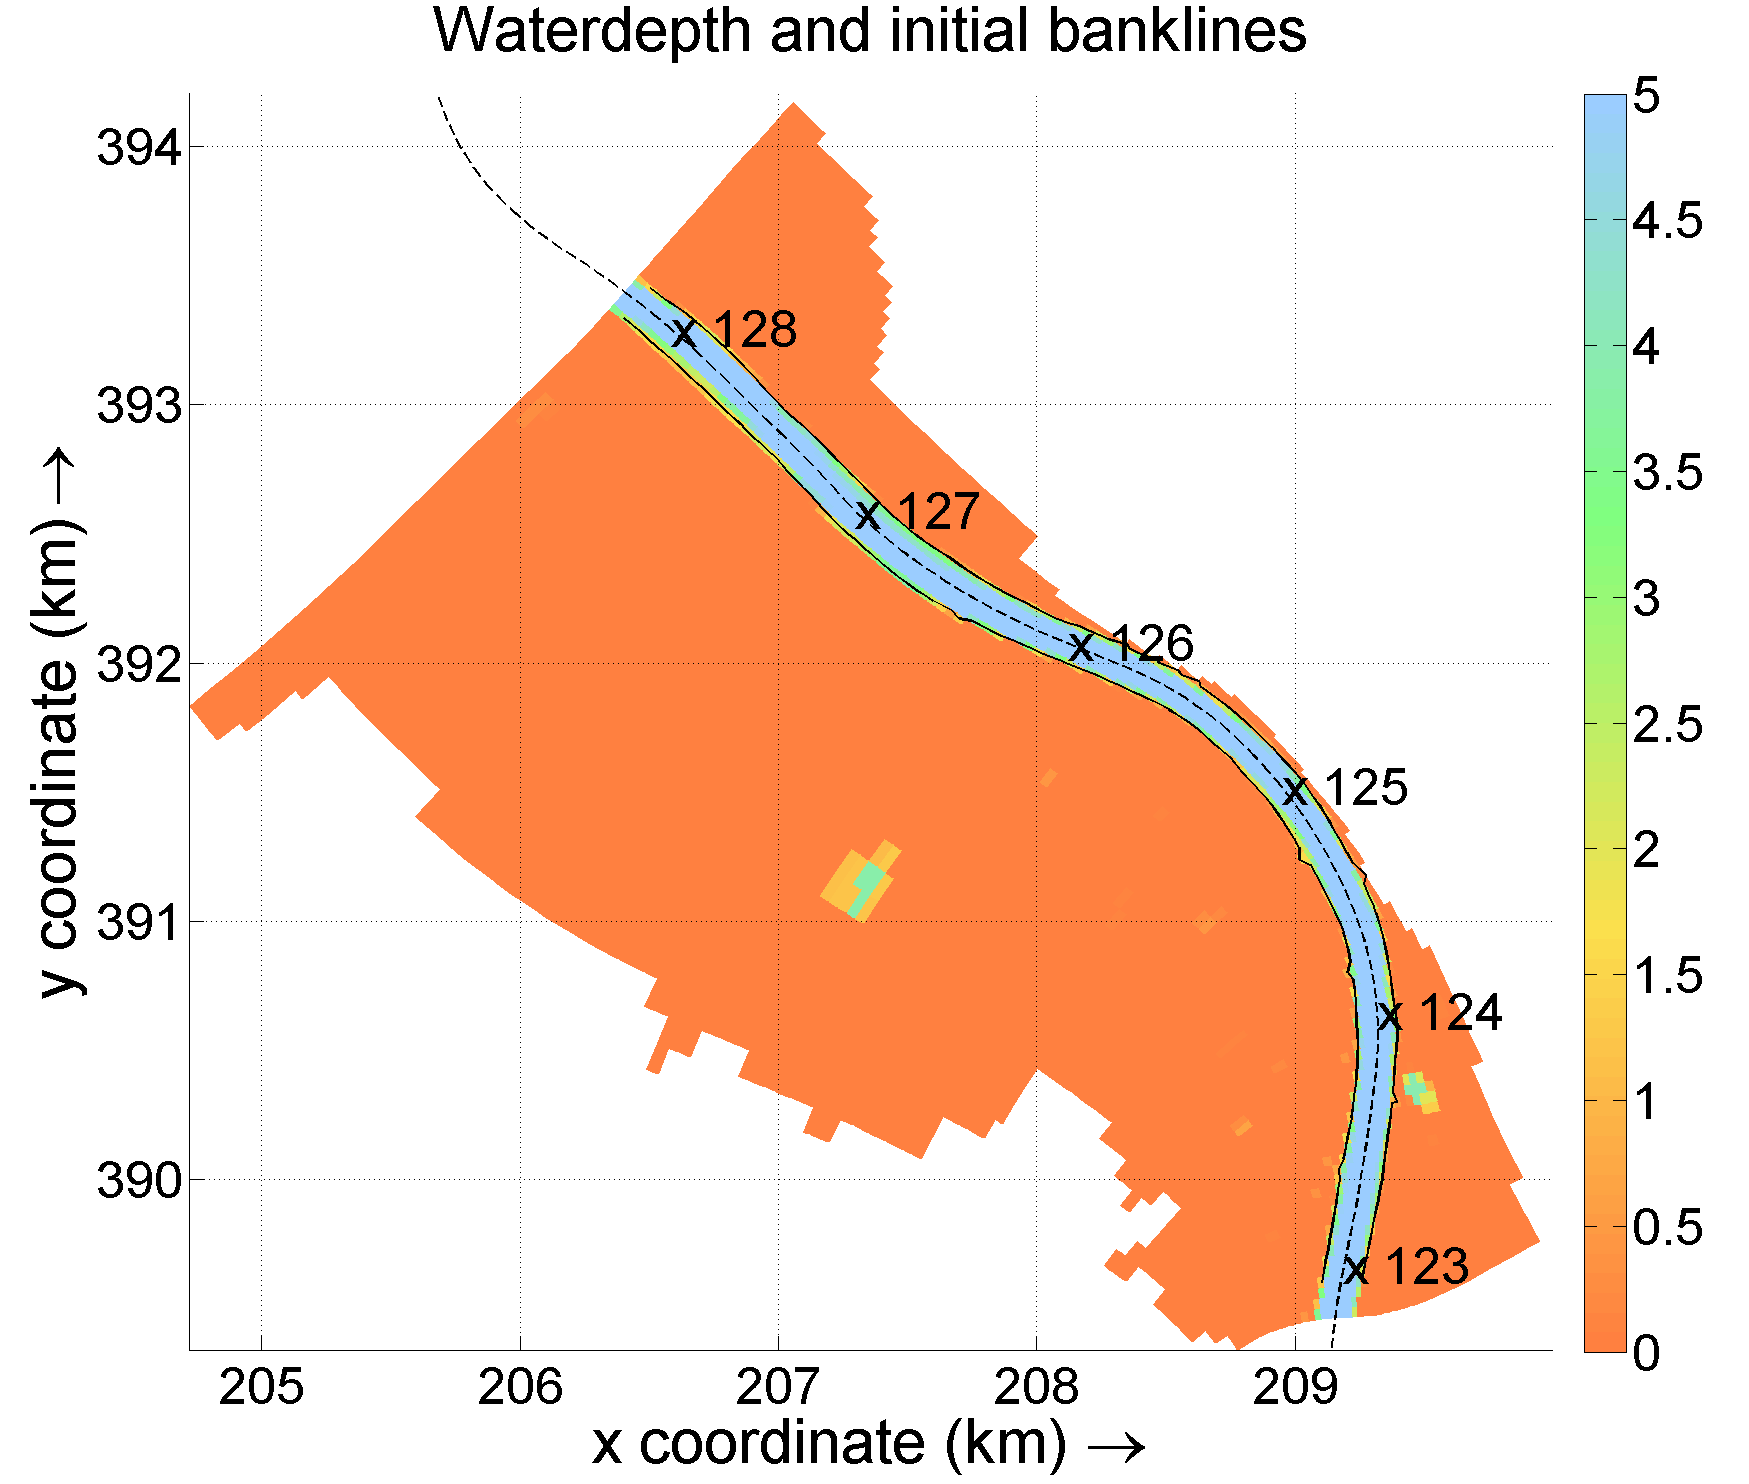
\includegraphics[width=\textwidth]{figures/Fig2-4.png}
\caption{Waterdepth, initial bank lines, river kilometers and fairway axis}
\label{Fig2.4}
\end{figure}

\begin{figure}
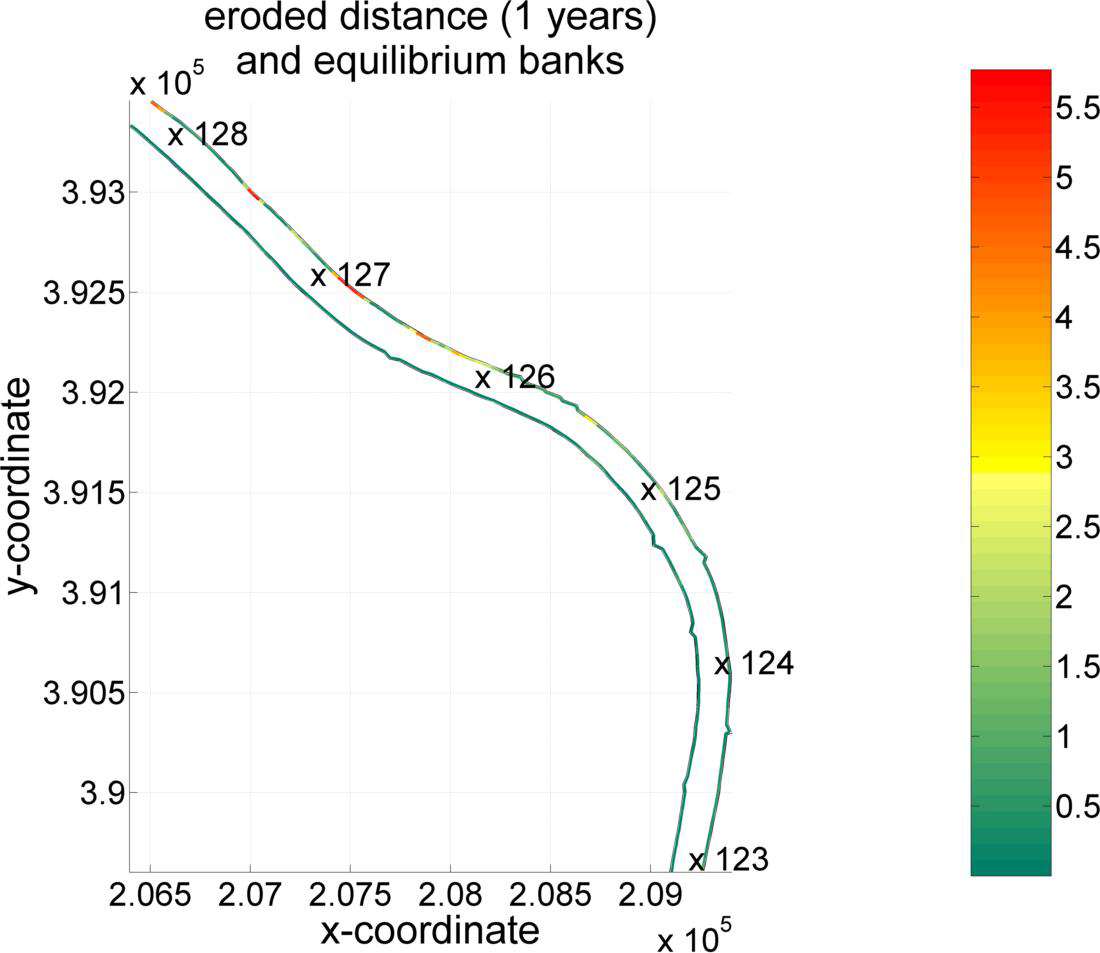
\includegraphics[width=\textwidth]{figures/Fig2-5.png}
\caption{Erosion sensitivity}
\label{Fig2.5}
\end{figure}

\begin{figure}
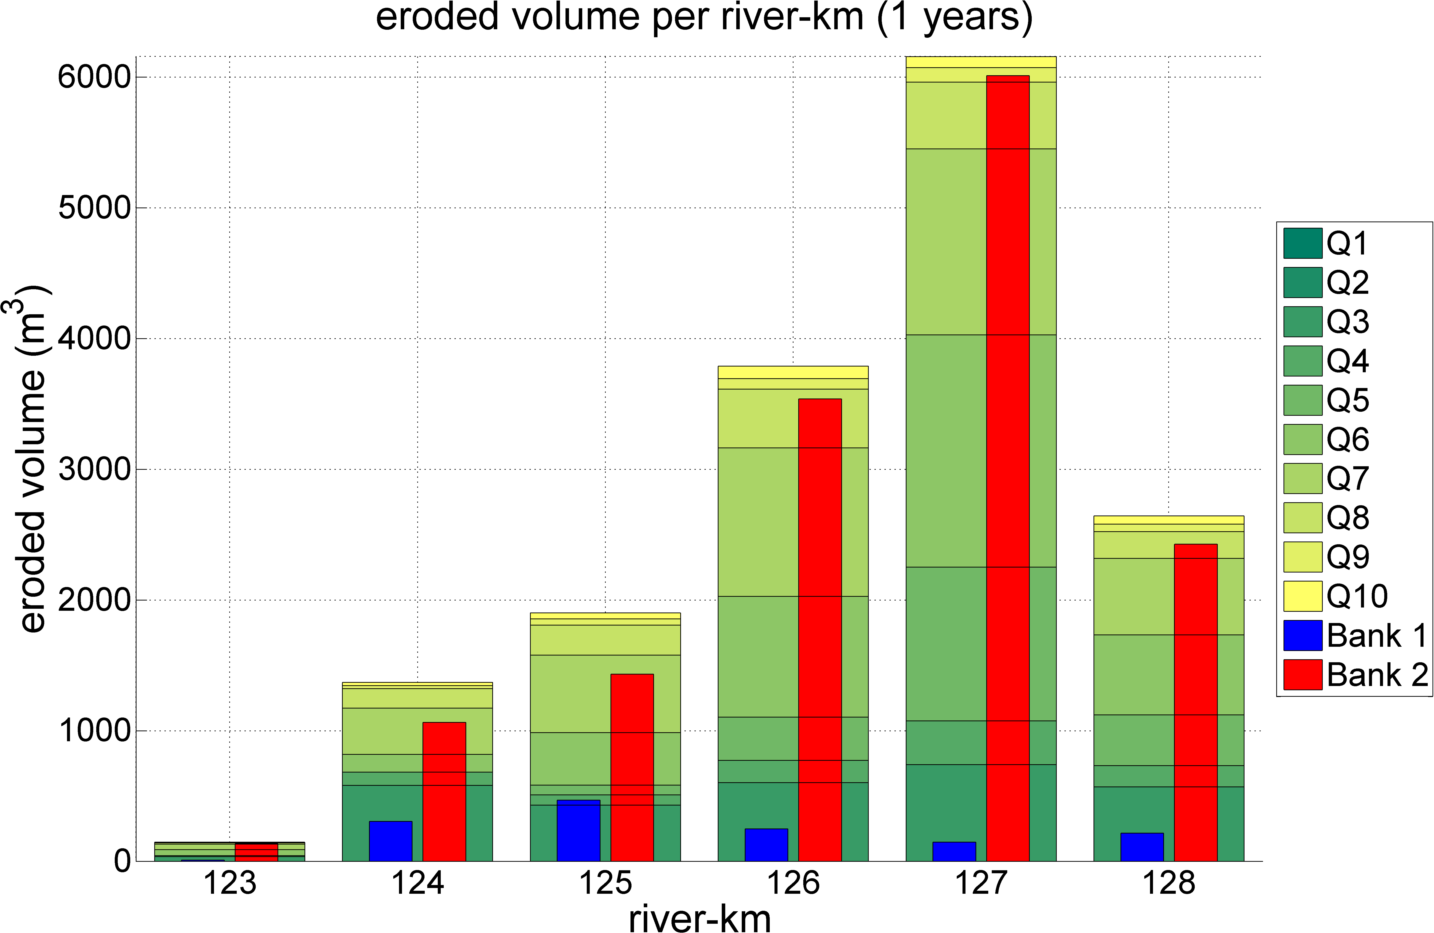
\includegraphics[width=\textwidth]{figures/Fig2-6.png}
\caption{Eroded volume at the end of the simulation period}
\label{Fig2.6}
\end{figure}

\begin{figure}
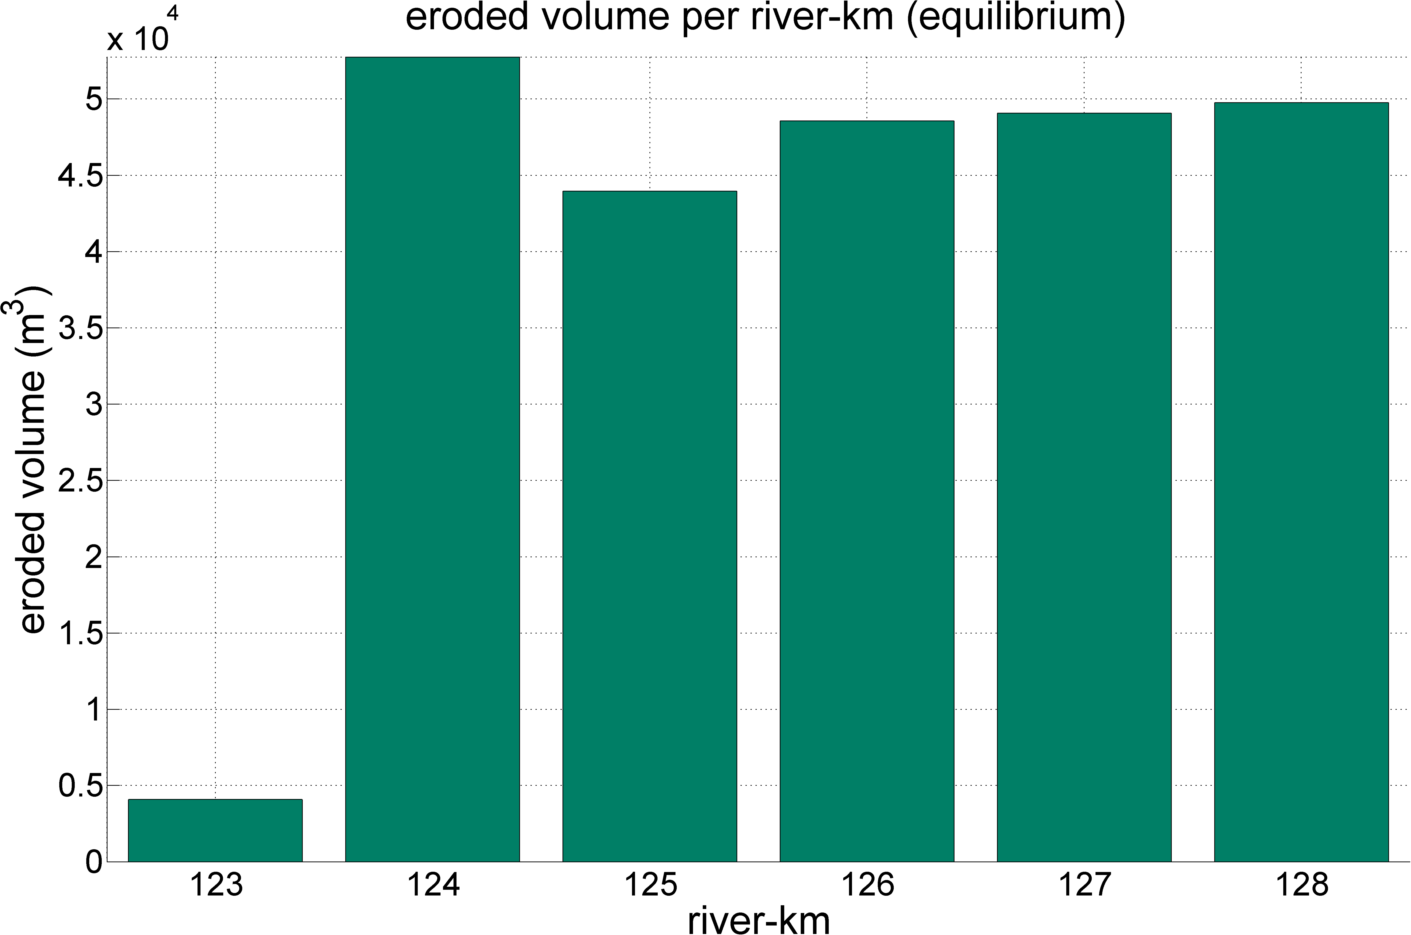
\includegraphics[width=\textwidth]{figures/Fig2-7.png}
\caption{Total erosion volume based on equilibrium bank line}
\label{Fig2.7}
\end{figure}

\begin{figure}
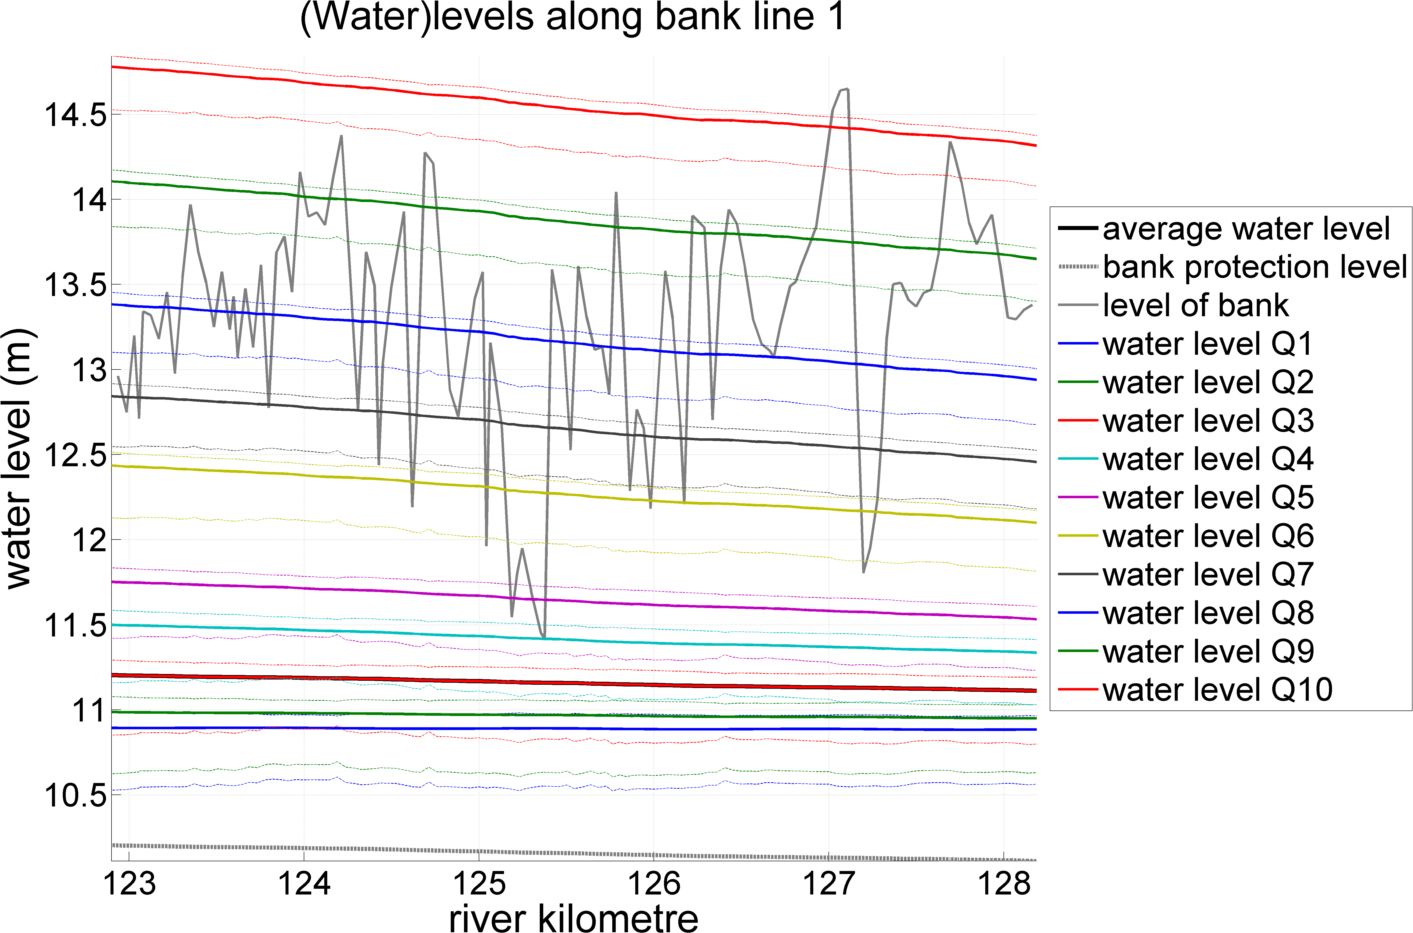
\includegraphics[width=\textwidth]{figures/Fig2-8.png}
\caption{Control figure for water levels of each discharge (bank line 1)}
\label{Fig2.8}
\end{figure}

\begin{figure}
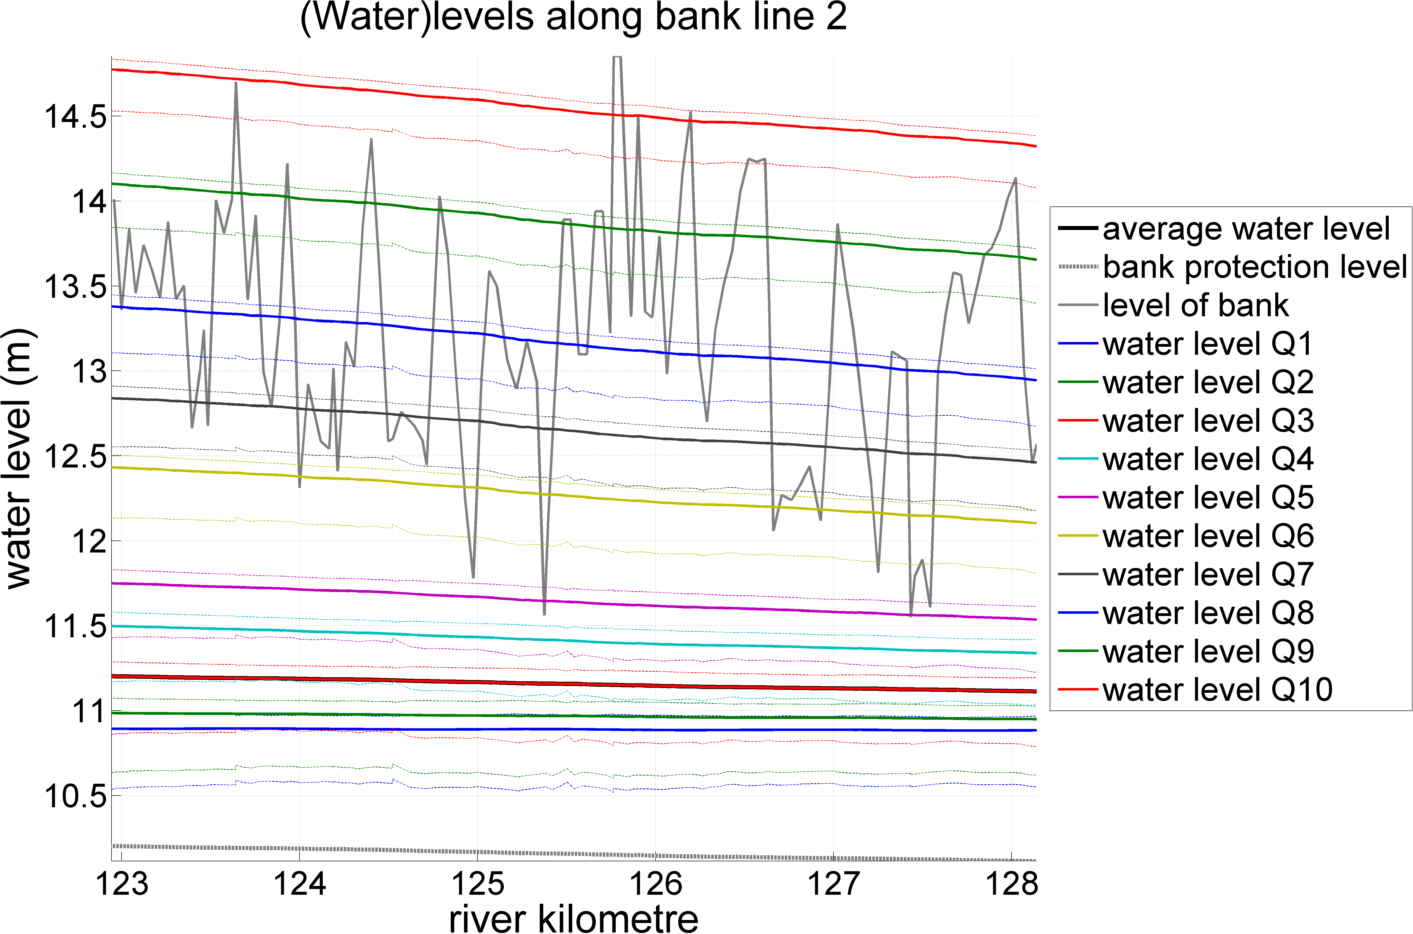
\includegraphics[width=\textwidth]{figures/Fig2-9.png}
\caption{Control figure for water levels of each discharge (bank line 2)}
\label{Fig2.9}
\end{figure}

\begin{figure}
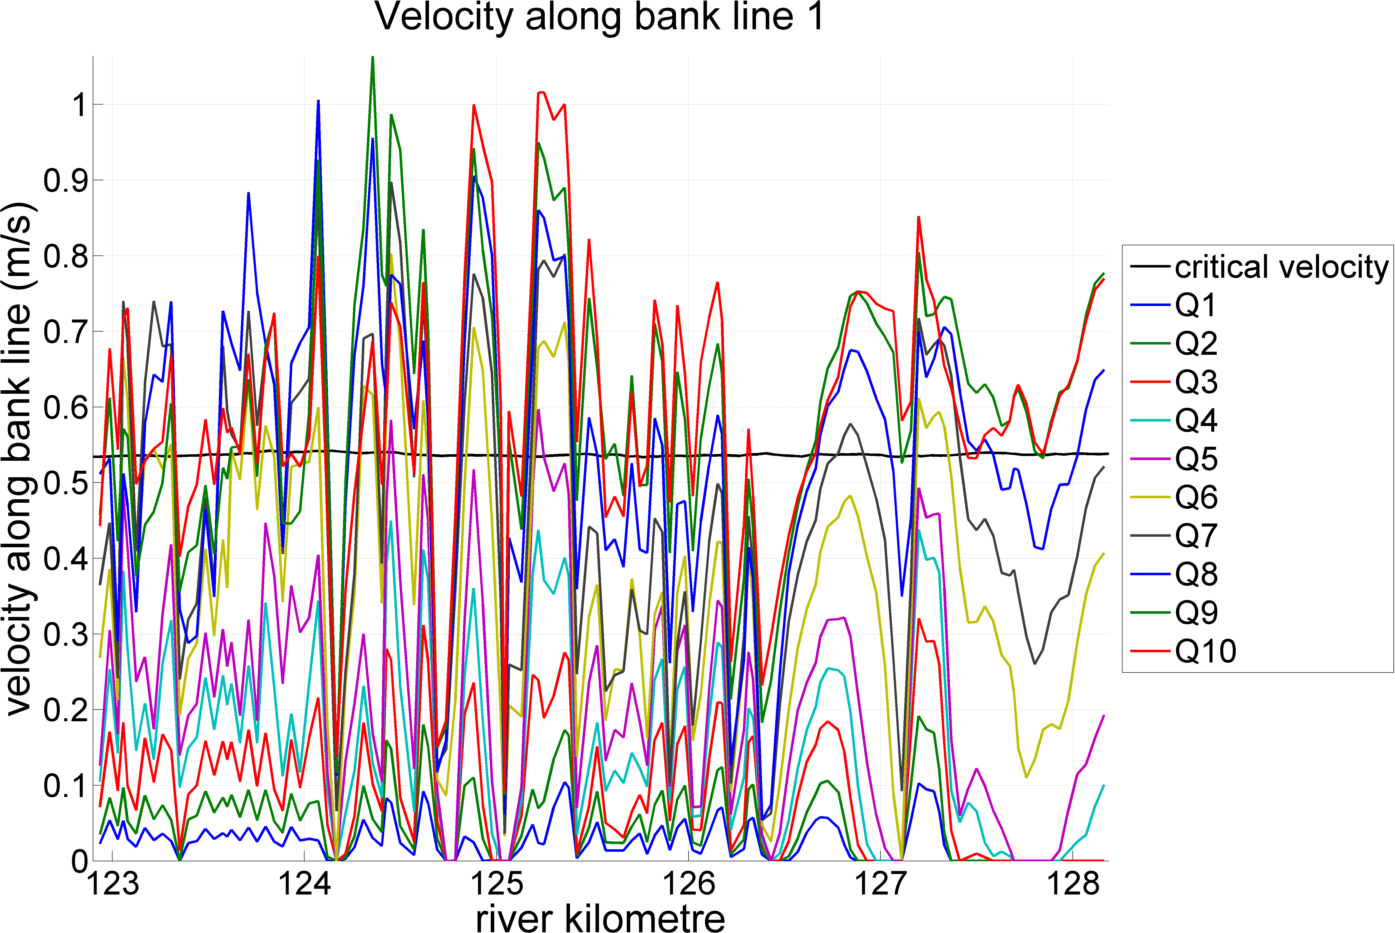
\includegraphics[width=\textwidth]{figures/Fig2-10.png}
\caption{No caption}
\label{Fig2.10}
\end{figure}

\begin{figure}
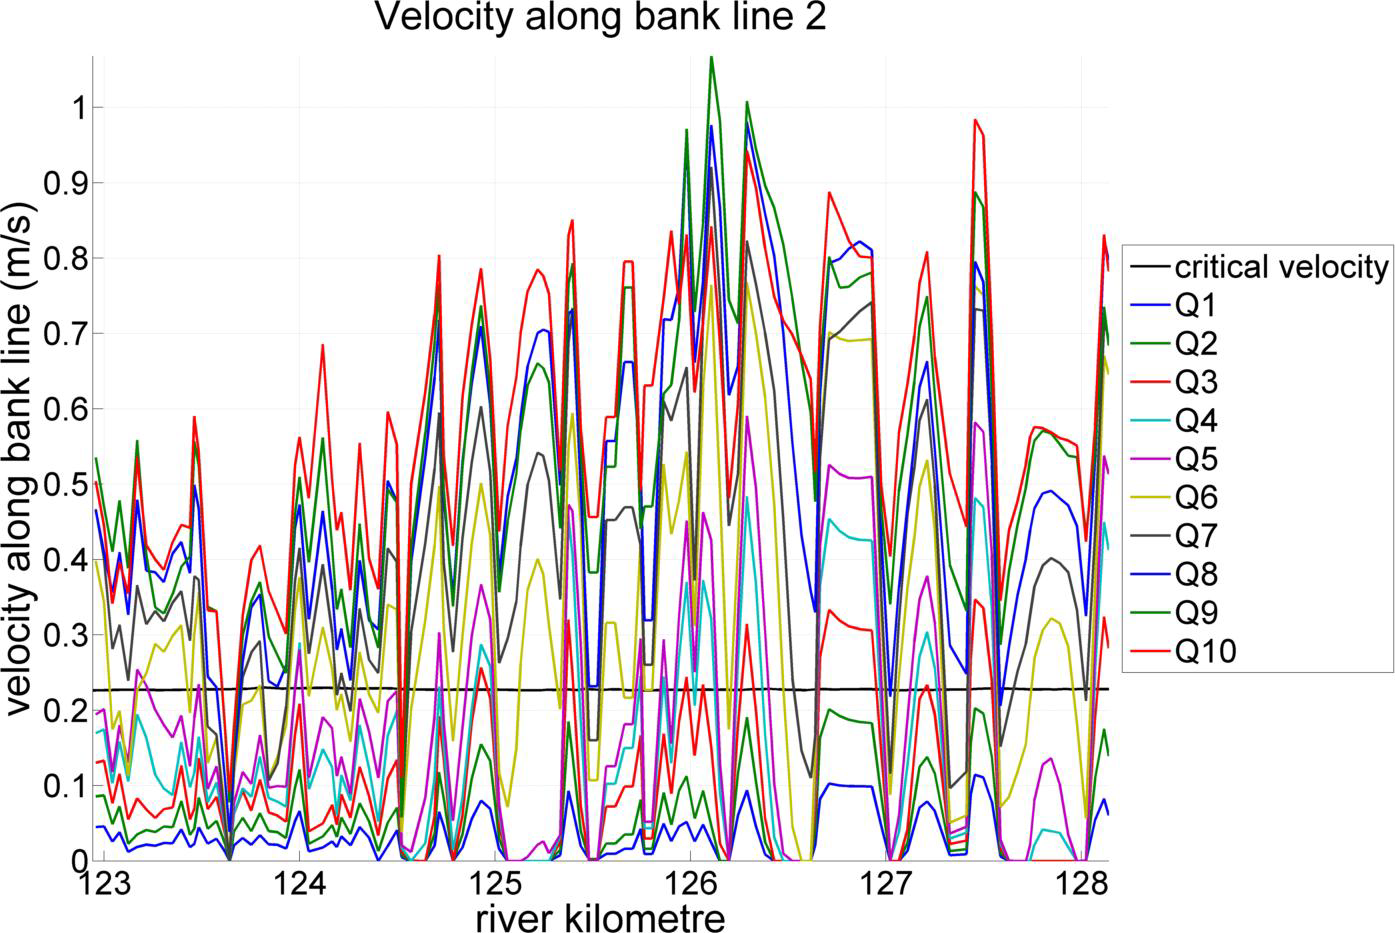
\includegraphics[width=\textwidth]{figures/Fig2-11.png}
\caption{No caption}
\label{Fig2.11}
\end{figure}

\begin{figure}
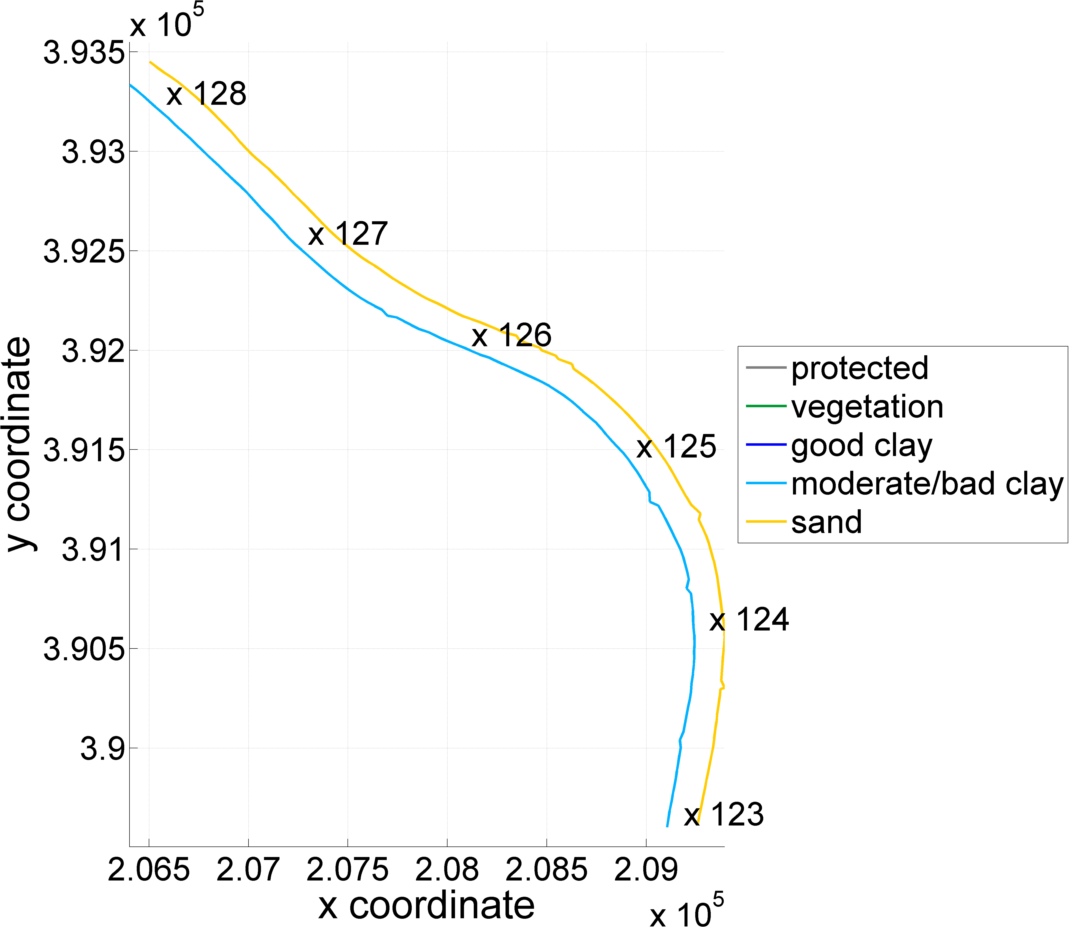
\includegraphics[width=\textwidth]{figures/Fig2-12.png}
\caption{Map with indication of applied bank type}
\label{Fig2.12}
\end{figure}

\begin{figure}
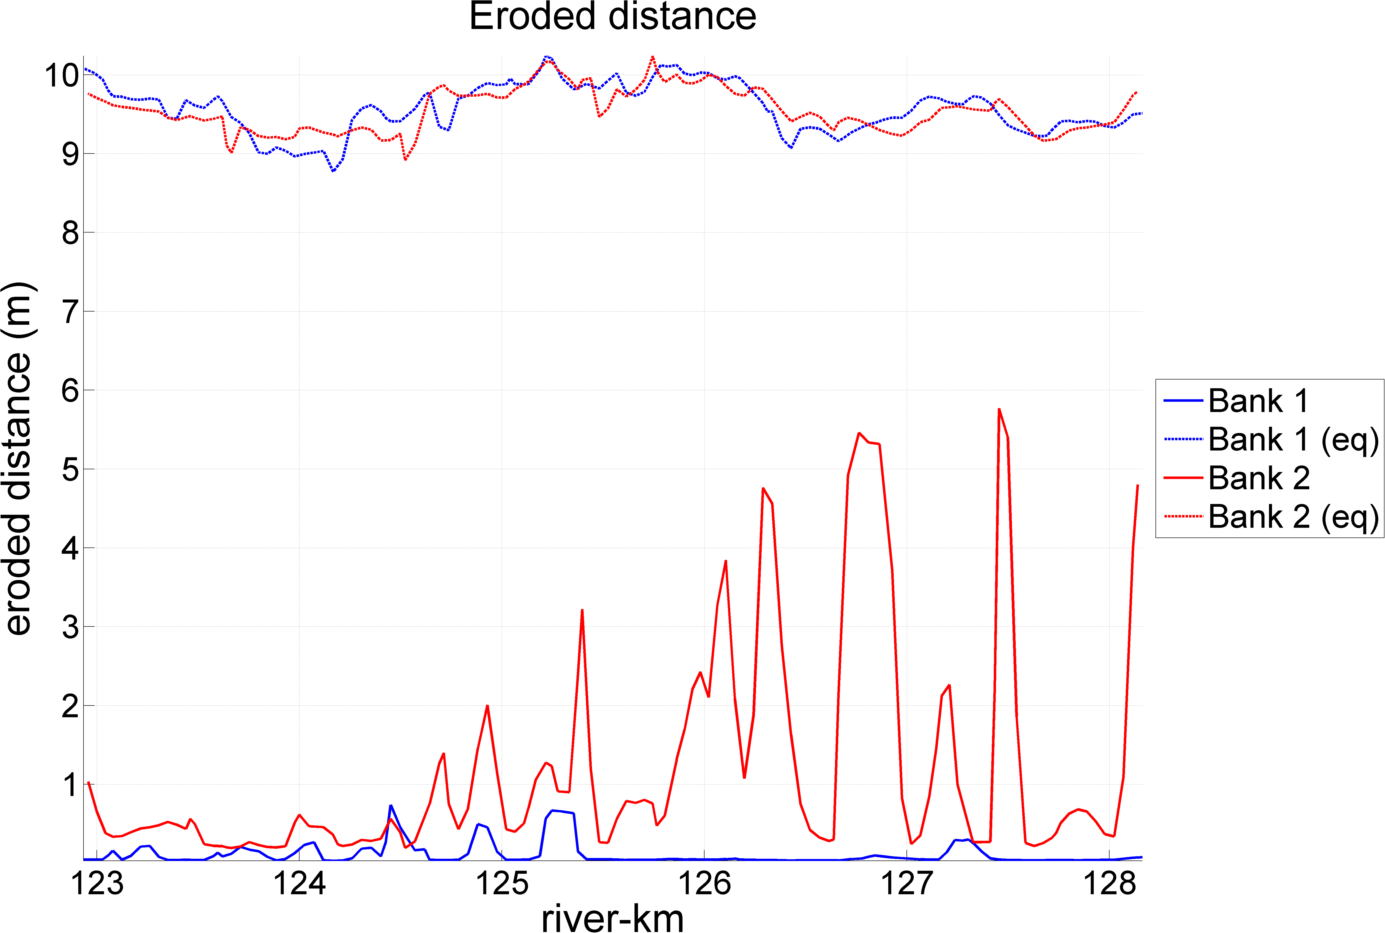
\includegraphics[width=\textwidth]{figures/Fig2-13.png}
\caption{Bank retreat at the end of the simulation period and for the equilibrium situation}
\label{Fig2.13}
\end{figure}

\chapter{Detecting and shifting the bank lines} \label{Chp:BankDetect}

This chapter describes the algorithms used for detecting (see \autoref{Sec:BankDetect}) and shifting (see \autoref{Sec:BankShift}) the bank lines.
The former happens in the 'banklines' detection step, whereas the latter happens in the 'bankerosion' analysis step after the bank erosion rates have been computed.
It also lists issues that you may run into during the detection step (see \autoref{Sec:DetectIssues}).

\section{Detecting the bank lines} \label{Sec:BankDetect}

The location of bank lines is determined by identifying the boundary between water (wet) and land (dry) at a reference discharge computed using \dflowfm.
The detection of the bank lines builds on the search lines provided as input to this step.
The model domain is first clipped to the area close to the search lines (i.e.~within the user specified search distance from the search line) to focus the bank detection algorithm on the areas of interest only.
Identifying the exact location of the bank lines starts by determining for each grid cell in the area of interest whether it has one (or more) bed levels $z_b$ (defined at the mesh nodes) above the water level $z_w$ in the grid cell and one (or more) bed levels below the water level (see \autoref{Fig:detect_step}).

\NumNote{\dfastbe currently only supports results of hydrodynamic simulations which use bed levels $z_b$ defined at grid nodes.
Simulations with bed levels defined in cell centres (tile depth) are thus not supported.}

\begin{figure}[!h]
\center
\resizebox{5cm}{!}{
   \input{figures/detect_step.pdf_tex}
}
\caption{The bank line determined by the transition from wet (bed levels $z_b$ below water level $z_w$) to dry (bed levels $z_b$ above water level $z_w$) per triangle}
\label{Fig:detect_step}
\end{figure}

For each of those grid cells, the sub-grid boundary between dry and wet parts is determined as the line along which the interpolated bed level equals the water level in the grid cell.
The line marking the zero water depth is a straight line in a triangle.
Cells with $N_c \ge 4$ corners are split into $N_c - 2$ triangles to arrive at a collection of only straight line segments.
The collection of all these line segments forms the basis of the final bank line, which is obtained by connecting the individual segments into long connected strands.
Subsequently, those bank line strands are selected that are closest to the river axis (to avoid selecting banks of floodplain lakes or side channels that are located close to the bank of interest).
The selected strands are finally connected across side channels entrances and other gaps to a continuous bank line for the whole reach of interest.
The resulting lines are written to a shape file for checking and use in the 'bankerosion' analysis step.

The found locations of the bank lines will clearly depend on the chosen discharge level.
However, as long as the discharge is within the main channel, the locations will be fairly consistent.

Generally, bank erosion only occurs along the main channel.
It is therefore possible to only take into account those cells that are within a certain distance from the predefined search lines.
This is also necessary when more than one bank line is present (as is common in rivers), because otherwise it is not clear which coordinates belong to one bank or the other.

The search lines should be defined in a simple text file consisting of x- and y- coordinates (\command{Line1}, ..., \command{LineN}, in the configuration file).
For the Dutch rivers the lines can be obtained from the Baseline 'oeverlijnen' for model schematisations up to Baseline 4.
For model schematisations of Baseline 5 and higher the 'oeverlijnen' can be obtained by:
%
\begin{enumerate}
\item merging the baseline section 1 and 2 polygon in one polygon feature,
\item transferring this polygon to a polyline feature,
\item cutting this feature into two separate banklines, and
\item transforming these lines to points along the lines with an interval of 10 metres.
\end{enumerate}

By using the 'oeverlijnen', or section 1-2 boundary from Baseline the tool only depicts the main channel.
Possible side channels, shortcuts or lakes will not be detected by the tool, see \autoref{Fig3.2}.
If they are important, extra lines can be added that indicate the location of the bank lines of these individual features.
For this the input \command{NBank} should be increased by the number of extra features and the location of the bank line file \command{LineN} should point to the new file(s) with the xy-coordinates of extra search line(s).
It should be noted that for the analysis of these extra bank sections the tool will still use the closest point \emph{of the main channel} for which the fairway and river axis have been specified which is likely not correct.
Hence a better approach is to run a separate analysis for these reaches in which provide appropriate lines for the fairway and river axis of those side channels.

Groynes are not detected as such by the tool, because they are typically defined on sub-grid level in the simulations, see \autoref{Fig3.3}.
The detected bank line is in this case following the banks within groyne sections.
This is an advantage, since possible bank erosion only takes place in the groyne sections and not along the groynes themselves.

\begin{figure}[!h]
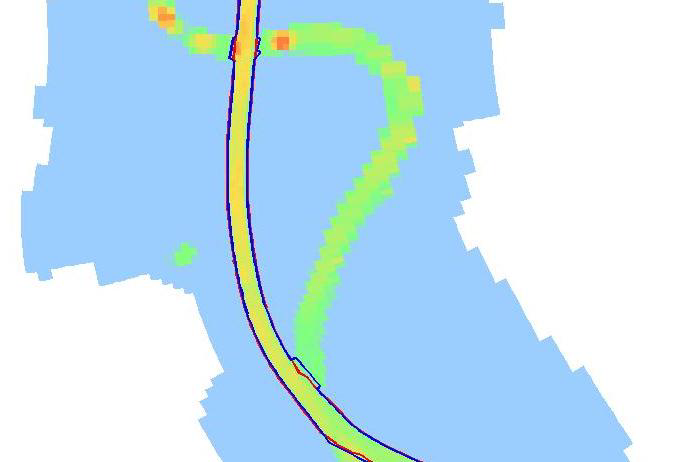
\includegraphics[width=\textwidth,height=7cm]{figures/Fig3-2.png}
\caption{Detection of bank lines at a shortcut in the Meuse river.
Red: Baseline 'section 1-2 boundary', Blue: detected bank line from WAQUA computation}
\label{Fig3.2}
\end{figure}

\begin{figure}[!hb]
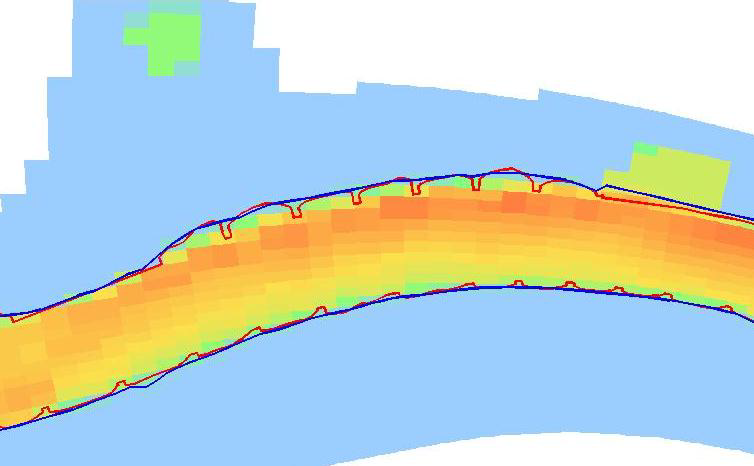
\includegraphics[width=\textwidth,height=7cm]{figures/Fig3-3.png}
\caption{Detection of a bank line close to groynes}
\label{Fig3.3}
\vspace{-0.75cm} 
\end{figure}
\clearpage

\section{Common issues with bank line detection} \label{Sec:DetectIssues}
It is advised to check the detected bank lines shown in the graphical output of the 'banklines' mode before continuing with the 'bankerosion' mode.
This section describes some common issues and their solutions.

\subsection{Detection of adjacent water body}
At some locations an adjacent water body is located within the given search distance from the predefined bank lines (parameter \command{Dlines}).
As a result the bank line of the adjacent water body is found, instead of the bank line of the main river channel.
As a result the initial bank line shows strange variations.
This is the case between kilometre 20 and 21 in \autoref{Fig_issue_bankline} location A.

\begin{figure}[!hb]
	\center
	\resizebox{15cm}{!}{
		\input{figures/detection_issue.pdf_tex}
	}
	\caption{Detection of the initial bank line close to adjacent water bodies}
	\label{Fig_issue_bankline}
\end{figure}

By decreasing the parameter \command{Dlines} you decrease the search distance from the predefined lines for determining the bank lines.
As a result, you decrease the chance that the bank line of an adjacent water  body is found.
However, you won't find a correct initial bank line if you make the parameter \command{Dlines} too small, this can be especially the case close to groins, at wide shallow areas or along banks with a relatively flat slope (see left bank between kilometre 22 and 23 in \autoref{Fig_issue_bankline} location B).

Another option is to edit the initial bank line manually by removing the points that fall in the adjacent water body, so only the points along the main channel remain.

\subsection{Irregularities in the detected bank line}
\autoref{Fig_issue_bankline} location C shows at the right outer bank after kilometre 22.5 a strange irregularity in the detected initial bank line.
This type of irregularities develop either by the detection of adjacent water body's, by the cut-off of connections with side channels (see \autoref{Fig_issue_bankline2}) or harbours or other irregularities along the bank.
It is advised to edit the initial bank line manually by removing some of the points so a smooth bank line along the main channel remains, because these irregularities influence the distance between the bank and the fairway and thus result in strange irregular patterns in wave heights and erosion along that bank.

\begin{figure}[!h]
	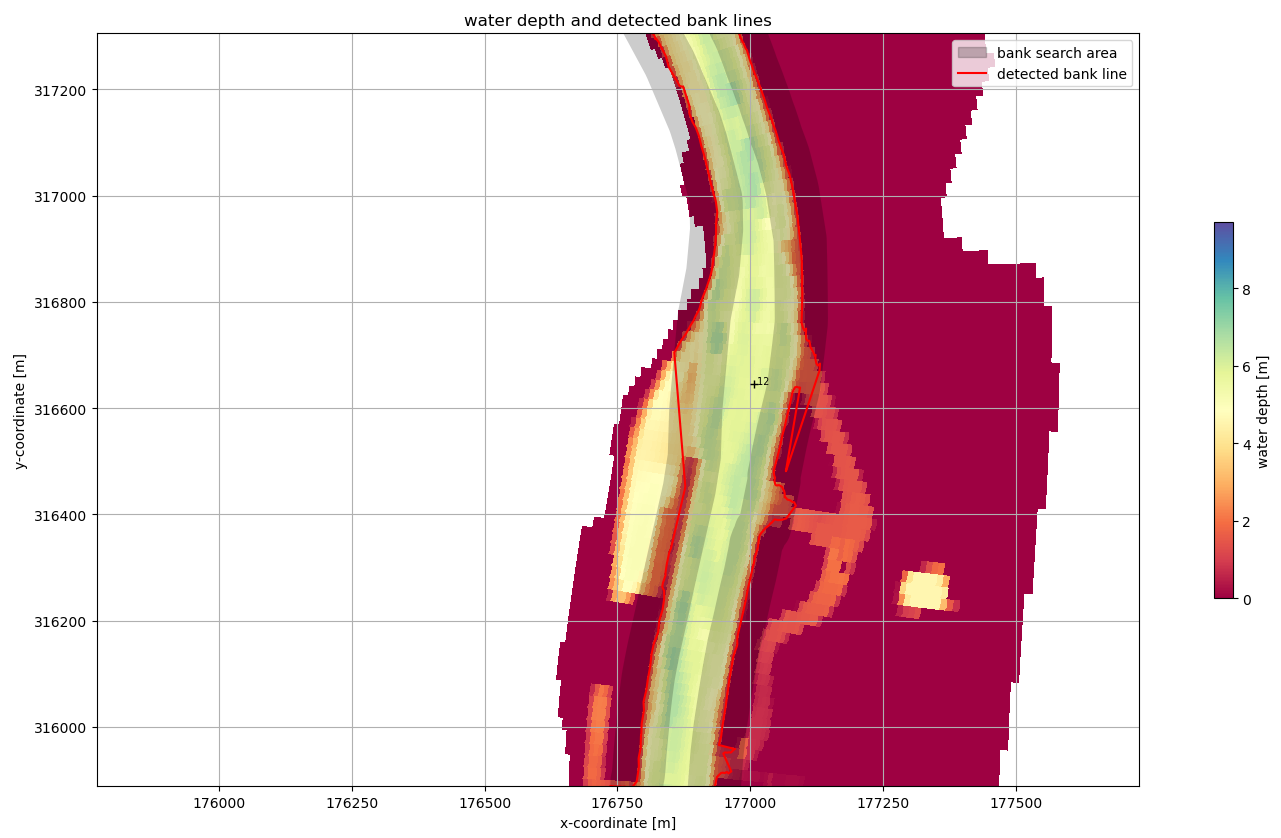
\includegraphics[width=\textwidth]{figures/detection_issue2.png}
	\caption{Detection of the initial bank line at the connection with a side channel}
	\label{Fig_issue_bankline2}
\end{figure}

\section{Shifting the bank lines} \label{Sec:BankShift}

The new location of the bank line is determined by shifting each bank line segment individually by its local erosion distance.
In the case of a concave bend the eroding segments move apart; a new bank segment is inserted connecting the two end points of the previously connected segments (see \autoref{Fig:erode_shift}, subplot a).
In case of a convex bend the eroding segments overlap; in this case the new bank line follows the outline of furthest erosion (see subplot b).

\begin{figure}[!h]
\center
\resizebox{12cm}{!}{
   \input{figures/erode_shift_step.pdf_tex}
}
\caption{Shifting a bank line first moves each line segment, and subsequently adds or removes segments as necessary}
\label{Fig:erode_shift}
\end{figure}

\chapter{Potential bank line shift and bank erosion} \label{Chp4}

Wanneer de ligging van de initiele oeverlijn bekend is, kan de potentiele oeverlijnverschuiving en oeverafslag worden bepaald.
De ontwikkelde oevererosiemodule is bedoeld als hulpmiddel om de potentiele oevererosie in te kunnen schatten en niet om de daadwerkelijke oevererosie te voorspellen.
Binnen de oevererosiemodule worden twee erosiemechanismen meegenomen: erosie door scheepsgolven en erosie door stroming.
Deze mechanismen worden in de volgende twee paragrafen verder uitgewerkt.
Verder wordt in paragraaf 0 uitgelegd hoe de oeverlijnverschuiving in zijn werk gaat.
De bepaling van het potentieel geerodeerd volume wordt uitgewerkt in \autoref{Sec4.4}.
In \autoref{Sec4.5} wordt uitgelegd hoe er kan worden omgegaan met een variabel afvoerniveau.
Het bepalen van de evenwichtsoever en het daarbij behorende geerodeerde volume wordt uitgelegd in \autoref{Sec4.6}.
Ten slotte worden enkele van de beperkingen van de oevererosiemodule aangestipt in \autoref{Sec4.7}.

\section{Determining potential erosion by ship waves} \label{Sec4.1}

Scheepsgolven zijn een van de belangrijkste factoren wat betreft oeverafslag (Verheij (2000))  en worden daarom als eerste oevererosiemechanisme meegenomen in de oevererosiemodule.
 De afleiding voor de erosieformulering voor scheepsgolven is overgenomen uit de BEM module (Verheij (2000), Stolker \& Verheij (2001b)) en definities van grootheden zijn gegeven in \autoref{Fig4.1}.

\begin{figure}
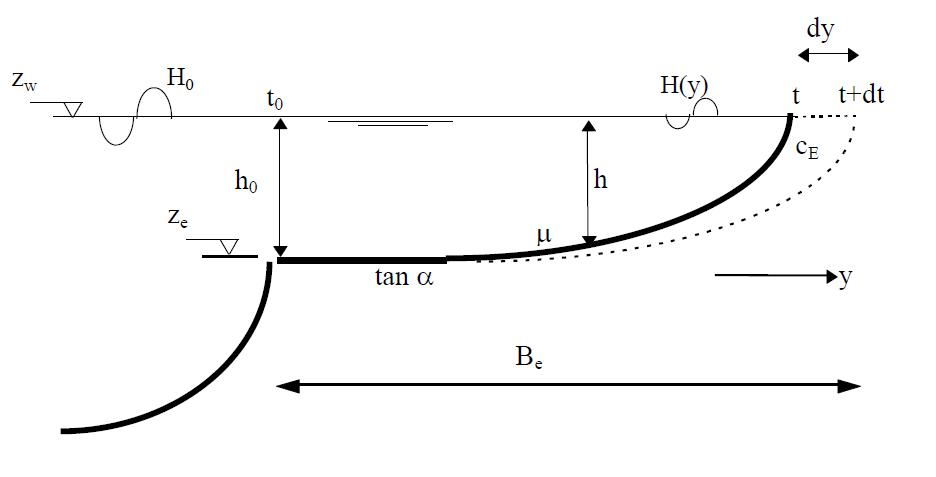
\includegraphics[width=8cm]{figures/Fig4-1.png}
\caption{Definities grootheden erosie door golven}
\label{Fig4.1}
\end{figure}

Op basis van grootschalige Deltagootproeven, waarbij diverse taluds van verschillende samenstelling werden belast onder loodrechte golfaanval, is afgeleid dat de erosiesnelheid kwadratisch toeneemt met de golfhoogte bij de oever:

\begin{equation}
\diff{y}{t} = c_E H^2
\label{Eq1.1}
\end{equation}

met:

\begin{symbollist}
\item[$y$] breedte van de afgekalfde oeverstrook \unitbrackets{m}
\item[$c_E$] sterkte coefficient voor oevermateriaal \unitbrackets{m\textsuperscript{-1}s\textsuperscript{-1}}
\item[$H$] golfhoogte bij de oever \unitbrackets{m}
\end{symbollist}

In het algemeen wordt verondersteld dat de afname van de golfhoogte via een negatieve e-macht is gerelateerd aan de breedte van de oeverstrook:

\begin{equation}
H = H_0 e^{-\mu y}
\label{Eq1.2}
\end{equation}

Hierin is:

\begin{symbollist}
\item[$H_0$] initiele golfhoogte aan het begin van de vooroever \unitbrackets{m}
\item[$\mu$] parameter voor golfdemping \unitbrackets{m\textsuperscript{-1}}
\end{symbollist}

Substitutie van \autoref{Eq1.2} in \autoref{Eq1.1} levert een differentiaalvergelijking op met de algemene oplossing:

\begin{equation}
\Delta n_\text{wave} = \frac{1}{2 \mu} ln ( 2 \mu c_E H_0^2 t + 1 )
\end{equation}

waarbij:

\begin{symbollist}
\item[$\Delta n_\text{wave}$] afstand waarmee de oeverlijn verschuift \unitbrackets{m}
\item[$t$] tijd \unitbrackets{s}
\end{symbollist}

Deze formule is toepasbaar voor zowel wind- als scheepsgolven.
In geval van scheepsgolven kan voor de tijd $t$ worden uitgegaan van de volgende relatie

\begin{equation}
t = T N n t_\text{eros} \text{ met } T = 0.51 \frac{v_s}{g} \text{.}
\end{equation}

waarbij:

\begin{symbollist}
\item[$T$] periode van de scheepsgolven \unitbrackets{s}
\item[$N$] aantal ongeladen schepen per jaar \unitbrackets{-}
\item[$n$] aantal golven per schip \textbf{-}
\item[$v_s$] vaarsnelheid schepen \unitbrackets{m/s}
\item[$g$] valversnelling 9.81 \unitbrackets{m/s\textsuperscript{2}}
\item[$t_\text{eros}$] beschouwde periode \unitbrackets{jaar}
\end{symbollist}

De waarde voor de initiele golfhoogte aan het begin van de vooroever $H_0$ kan met behulp van formules zoals uit DIPRO worden berekend aan de hand van het type maatgevende schepen, hun vaarsnelheid en diepgang, de afstand tussen de vaargeul en de oever en de waterdiepte (zie Bijlage A5A).

De parameter $\mu$ kan worden gebruikt om de invloed in rekening te brengen van de vorm van de vooroever op de golfdemping, maar ook het dempende effect van vooroeverconstructries, vegetaties, en afzettingen van oevermateriaal.
In de oevererosiemodule wordt alleen het effect van de helling van de vooroever op de golfdemping meegenomen.
De dempingsterm voor glooiende bodemhellingen wordt als volgt bepaald (Verheij (2000)):

\begin{equation}
\mu_\text{vo} = \frac{\tan \alpha}{H_0}
\end{equation}

Waarbij $\tan \alpha = \frac{1}{n}$ voor een vooroever met een helling van 1:$n$ (zie ook \autoref{Fig4.1}).
Uitgaande van een initiele golfhoogte $H_0 = 0.4$ leidt een helling tussen de 1:100 en 1:20 tot waarden van $\mu_\text{vo}$ liggend tussen 0.025 en 0.125.
In \autoref{Fig4.2} is een voorbeeld gegeven van de invloed van de dempingsparameter $\mu_\text{vo}$ op de oevererosie door golven.

\begin{figure}
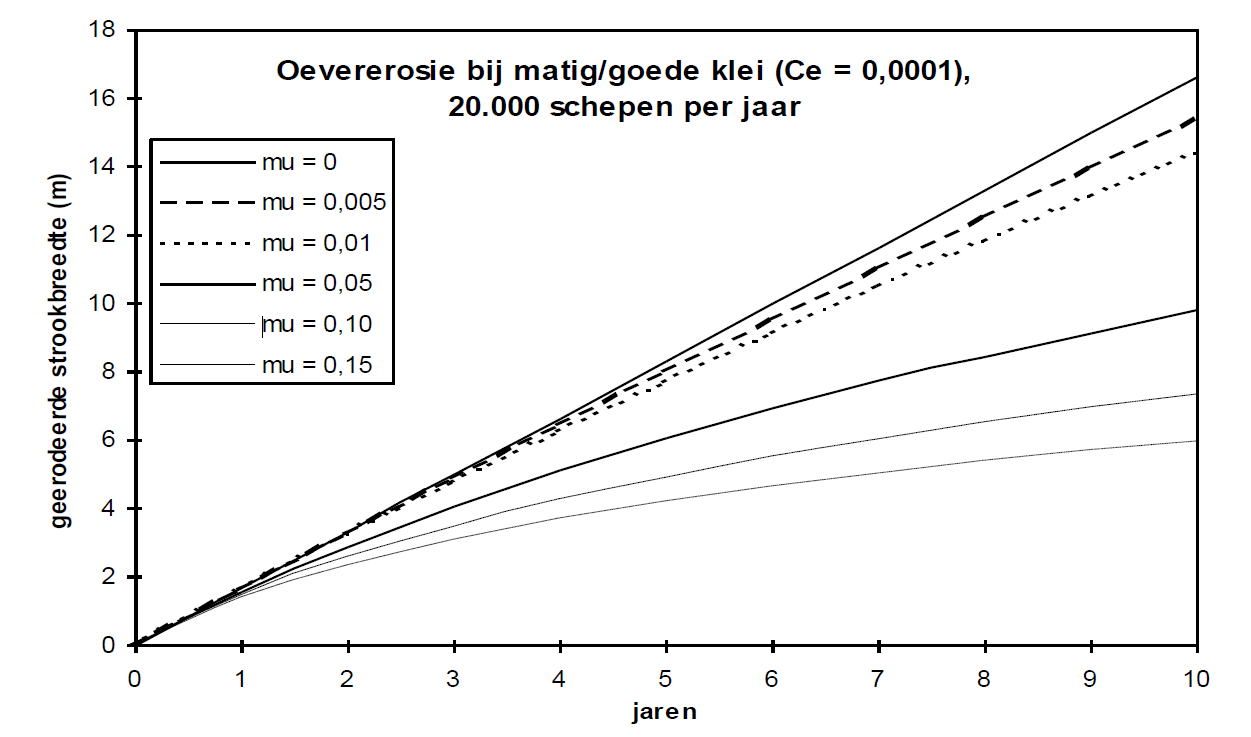
\includegraphics[width=\textwidth]{figures/Fig4-2.png}
\caption{Voorbeeld van oevererosie door golven voor matig/goede klei.}
\label{Fig4.2}
\end{figure}

Naast de golfdemping door de helling van de vooroever kunnen de inkomende golven ook worden gedempt door de begroeiing.
Voor golfdemping door riet is de volgende relatie beschikbaar

\begin{equation}
\mu_r = 8.5 \cdot 10^{-4} N_r^{0.8}
\end{equation}

met $N_r$ de rietstengeldichtheid (aantal stengels per vierkante meter).
De totale golfdemping door de helling van de vooroever en riet wordt dan

\begin{equation}
\mu_\text{tot} = \mu_\text{vo} + \mu_r
\end{equation}

De waarde voor de sterkte van het oevermateriaal $c_E$ hangt af van de samenstelling van de oever en kan ruimtelijk varieren.
Waarden voor $c_E$ voor verschillende oeversamenstellingen zijn te vinden in \autoref{Tab4.1}.
Per oeverlijn moet in een tekstbestand worden aangegeven uit welke klasse het oevermateriaal bestaat voor een bepaald riviertraject.

\begin{table}
\begin{tabular}{llll}
Klasse & Grond & $c_E$ \unitbrackets{m\textsuperscript{-1} s\textsuperscript{-1}} & $\tau_c$ \unitbrackets{Pa} \\ \hline
0 & Beschermde oeverlijn & 0 & $\infty$ \\
1 & Begroeide oeverlijn & 0.02 10\textsuperscript{-4} & 95 \\
2 & Goede klei & 0.6 10\textsuperscript{-4} & 3 \\
3 & Matig / slechte klei  & 2 10\textsuperscript{-4} & 0.95 \\
4 & Zand & 12.5 10\textsuperscript{-4} & 0.15 \\ \hline
\end{tabular}
\caption{Klassenindeling grondsoorten oevererosiemodule}
\label{Tab4.1}
\end{table}

\section{Determining potential erosion by currents} \label{Sec4.2}

Naast oeverafslag door scheepsgolven kan ook een sterke stroming langs de oever zelf zorgen voor oevererosie.
Dit mechanisme wordt ook meegenomen in de oevererosiemodule.
Voor elke oeverlijn kan de potentiele oevererosie door stroming bij een bepaalde afvoer $Q$ worden bepaald aan de hand van de volgende formule:

\begin{equation}
\Delta n_\text{flow} = E \left ( \frac{u_b^2}{u_c^2} - 1 \right ) t_\text{eros}
\end{equation}

met

\begin{symbollist}
\item[$\Delta n_\text{flow}$] afstand waarmee de oeverlijn verschuift in periode $t_\text{eros}$ \unitbrackets{m}
\item[$E$] erosiecoefficient van de oever \unitbrackets{m/s}
\item[$u_b$] stroomsnelheid langs de oeverlijn \unitbrackets{m/s}
\item[$u_c$] kritische stroomsnelheid voor erosie \unitbrackets{m/s}
\item[$t_\text{eros}$] beschouwde periode \unitbrackets{s}
\end{symbollist}

De erosiecoefficient wordt bepaald volgens:

\begin{equation}
E = \alpha \sqrt{\tau_c}
\end{equation}

met $\alpha$ = 2 10\textsuperscript{-7} \unitbrackets{m\textsuperscript{-3/2} kg\textsuperscript{1/2}} en $\tau_c$ \unitbrackets{N/m\textsuperscript{2}} de kritische schuifspanning voor erosie.
Deze waarde voor de erosiecoefficient is vergelijkbaar met erosiecoefficienten die in de literatuur gevonden worden (bijv.
Crosato, 2007).

Deze relatie tussen de kritische schuifspanning en de erosiecoefficient is echter niet universeel en daarom is het ook mogelijk om de erosiecoefficient als afzonderlijke invoer op te geven.

Voor de kritische stroomsnelheid voor erosie geldt:

\begin{equation}
u_c = \sqrt{\frac{\tau_c}{\rho} \frac{C^2}{g}}
\end{equation}

met $C$ \unitbrackets{m\textsuperscript{1/2}/s} de Chezy coefficient voor hydraulische ruwheid.
De waarde voor de Chezy coefficient wordt overgenomen uit de D-Flow FM berekening.

De stroomsnelheid langs de oever wordt bepaald aan de hand van de stroomsnelheid uit D-Flow FM.
De waarde voor de kritische schuifspanning voor erosie, $\tau_c$ , is gerelateerd aan de sterkte coefficient voor oevermateriaal, $c_E$ , zoals beschreven in Bijlage B)

\section{Total bank shift} \label{Sec4.3}

De totale oeverlijnverschuiving wordt gevonden door te sommeren over de oeverlijnverschuivingen veroorzaakt door de verschillende erosiemechanismen:

\begin{equation}
\Delta n = \Delta n_\text{flow} + \Delta n_\text{wave}
\end{equation}

De nieuwe locatie van een oeverlijn wordt bepaald door elk lijnsegment te verplaatsen volgens zijn lokale verschuiving.
De nieuwe locatie van een punt van de oeverlijn wordt gevonden door het snijpunt van de twee naburige segmenten te berekenen, zie \autoref{Fig4.3}.
Echter, in sommige situaties kan dit resulteren in erg grote verplaatsingen van punten, vooral wanneer naburige segmenten bijna in elkaars verlengde liggen.
In deze gevallen worden eerst twee locaties bepaald gebaseerd op de verplaatsing van elk van de naburige segmenten (rode stippen in \autoref{Fig4.4}).
De uiteindelijke locatie van een punt wordt dan bepaald door het gemiddelde van deze twee punten te nemen (groene stip in \autoref{Fig4.4}).


\begin{figure}
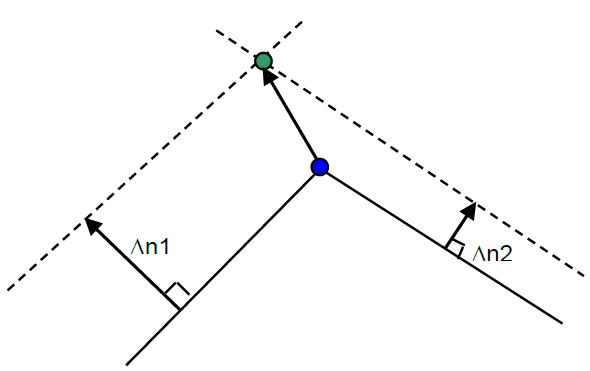
\includegraphics[width=6cm]{figures/Fig4-3.png}
\caption{Het verschuiven van een oeverlijn gebaseerd op het snijpunt van twee lijnsegmenten.
Blauw: oorspronkelijke locatie, Groen: nieuwe locatie}
\label{Fig4.3}
\end{figure}

\begin{figure}
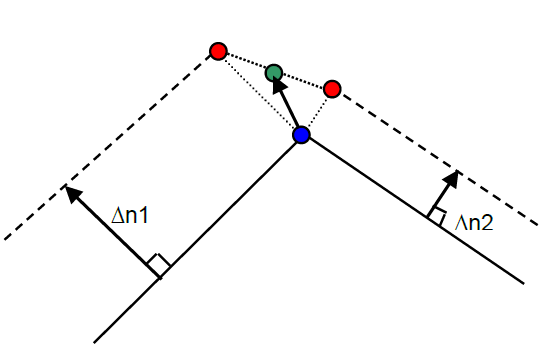
\includegraphics[width=5cm]{figures/Fig4-4.png}
\caption{Het verschuiven van een oeverlijn gebaseerd op de gemiddelde verplaatsing van twee lijnsegmenten.
Blauw: oorspronkelijke locatie, Rood: nieuwe locatie gebaseerd op individuele segmenten, Groen: nieuwe locatie (gemiddelde van de rode punten).}
\label{Fig4.4}
\end{figure}

Om numerieke problemen te voorkomen worden te kleine oeverlijnsegementen samengevoegd met hun buren.

\section{Potential bank erosion volume} \label{Sec4.4}

Naast de potentiele oeverlijnverschuiving is ook het potentiele volume aan sediment dat vrijkomt door erosie van belang.
Deze hoeveelheid sediment komt uiteindelijk in de rivier terecht, wat gevolgen kan hebben voor de bodemligging en eventueel noodzaak kan geven tot extra baggerwerkzaamheden.
Het potentiele volume aan sediment dat vrijkomt door erosie kan worden afgeschat door

\begin{equation}
V_\text{afslag} = ( \delta h_\text{bov} + \delta h_\text{ben} ) \Delta n
\end{equation}

waarbij $\Delta n$ de totale oeverlijnverschuiving en $\delta h$ het invloedsgebied van het afslagproces (boven en onder de waterspiegel).

Er wordt verondersteld dat de oever in zijn geheel terugschrijdt en daarom geldt voor het invloedsgebied boven de waterspiegel:

\begin{equation}
\delta h_\text{bov} = z_\text{oever} - z
\end{equation}

met

\begin{symbollist}
\item[$z$] waterspiegelniveau \unitbrackets{m}
\item[$z_\text{oever}$] niveau bovenkant steiloever \unitbrackets{m}
\end{symbollist}

De grootte van het invloedsgebied onder de waterspiegel wordt bepaald door de golfhoogte en het niveau tot waar het stortsteen blijft liggen.
Hiervoor wordt de volgende relatie gebruikt:

\begin{equation}
\delta h_\text{ben} = \min ( z-z_\text{ss}, 2 H )
\end{equation}

waarbij:

\begin{symbollist}
\item{$z$} waterspiegelniveau \unitbrackets{m}
\item{$z_\text{ss}$} niveau bovenkant stortsteen \unitbrackets{m}
\item{H} golfhoogte bij de oever \unitbrackets{m}
\end{symbollist}

In \autoref{Fig4.5} is geschematiseerd weergegeven wat het geerodeerd volume is voor verschillende situaties van de waterstand.


\begin{figure}
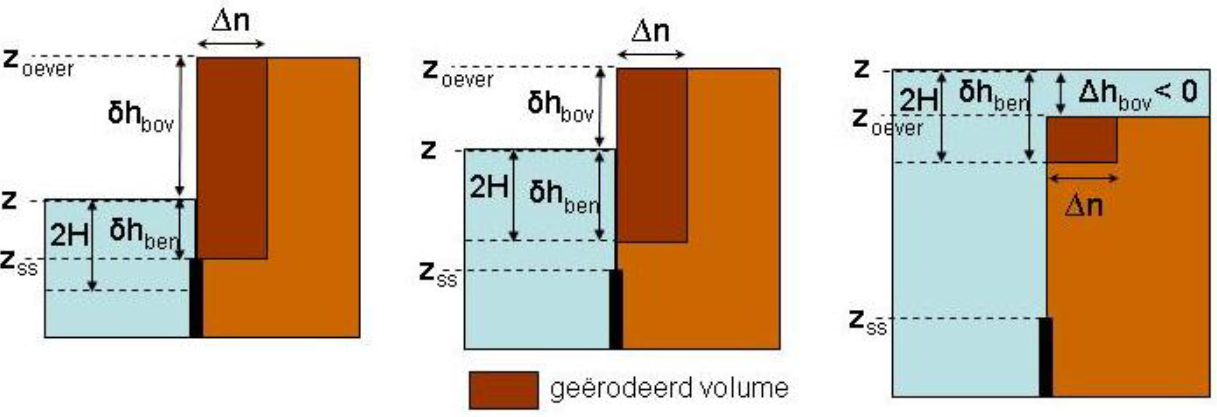
\includegraphics[width=\textwidth]{figures/Fig4-5.png}
\caption{Geerodeerd volume voor verschillende situaties van de waterstand.}
\label{Fig4.5}
\end{figure}

De terugschrijding van de oever wordt volledig bepaald door de oeverafslag, ongeacht of het materiaal dat voor de oever op de bodem terecht komt meteen wordt afgevoerd of niet.
Het afgeslagen materiaal beinvloedt wel de vervolgerosie, omdat het in zekere zin de oever beschermt.
De invloed hiervan kan niet worden bepaald door alleen een sedimentbalans op te stellen a.d.h.v.
een sedimenttransportformule, omdat soms grote hompen klei blijven liggen die eerst moeten desintegreren voordat de stroming ze kan meenemen.
De invloed van het afgeslagen materiaal op de golfhoogte (en daardoor de erosie door scheepsgolven) kan wel worden meegenomen door de parameter voor golfdemping, $\mu$, te verhogen.

\section{Variable discharge} \label{Sec4.5}

Het meenemen van een variabele afvoer is mogelijk door de afvoerverdeling te schematiseren met een hydrograaf.
Deze hydrograaf bestaat uit $n_Q$ afvoerniveaus en hun bijbehorende kans op voorkomen.
Voor elk afvoerniveau wordt een aparte D-Flow FM-berekening uitgevoerd.
Uit deze D-Flow FM simulaties kunnen dan de stroomsnelheid langs de oeverlijn en het niveau van de waterspiegel worden afgeleid.
Hierbij wordt er vanuit gegaan dat in ieder geval de afvoer wordt meegenomen die is gebruikt om de initiele oeverlijn te bepalen (de gemiddelde afvoer).

Vervolgens worden oeverlijnverschuivingingen voor de afzonderlijke afvoerniveaus bepaald en deze worden daarna gewogen gesommeerd aan de hand van de kans van voorkomen van het betreffende afvoerniveau.
Voor elk afvoerniveau $Q_i$ wordt dus eerst de totale erosie $\Delta n ( Q_i )$ voor die afvoer bepaald, die bestaat uit een deel veroorzaakt door scheepsgolven en een deel veroorzaakt door stroming.

Een variabele afvoer betekent dat ook het niveau van de waterspiegel tijdsafhankelijk is en daarmee de locatie waar de oevererosie optreedt.
In de oevererosiemodule wordt echter uitgegaan van een initiele oeverlijn (behorende bij een gemiddelde afvoer).
De mate van erosie van deze lijn varieert echter wel met de afvoer.


\subsection{Erosion by ship waves}

Een varierend afvoerniveau zorgt voor een varierend niveau van de waterspiegel.
De initiele oeverlijn is echter alleen onderhevig aan erosie door golven bij een gegeven afvoer $Q_i$ als de hoogte van de lijn in het invloedsgebied [$z(Q_i) - 2 H$, $z(Q_i) + \frac{1}{2} H$] ligt, waarbij $H$ de golfhoogte bij de oever en $z(Q_i)$ het niveau van de waterspiegel bij afvoer $Q_i$.
In de voorbeelden weergegeven in \autoref{Fig4.6} is de oeverlijn dus alleen onderhevig aan erosie door golven bij afvoerniveaus $Q_2$ en $Q_3$.
Of een oeverlijn binnen het invloedsgebied ligt waarin erosie door golven moet worden meegenomen, kan plaatsafhankelijk zijn.
In het benedenstroomse gebied liggen de waterniveaus bij verschillende afvoeren in het algemeen dichter bij elkaar dan bovenstrooms en ook vlakbij een stuw met een opgegeven stuwpeil kan het waterniveau redelijk constant blijven voor verschillende afvoeren.

\begin{figure}
\begin{tabular}{p{6cm}p{6cm}}
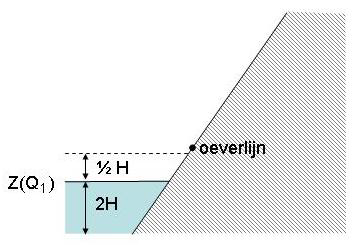
\includegraphics[width=5cm]{figures/Fig4-6a.png} \linebreak
a) &
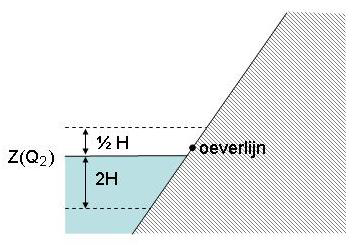
\includegraphics[width=5cm]{figures/Fig4-6b.png} \linebreak
b) \\
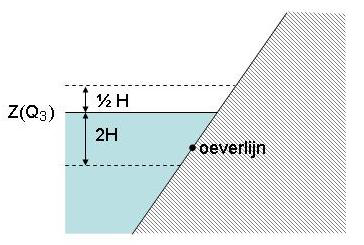
\includegraphics[width=5cm]{figures/Fig4-6c.png} \linebreak
c) &
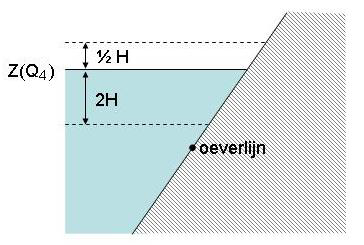
\includegraphics[width=5cm]{figures/Fig4-6d.png} \linebreak
d) \\
\end{tabular}
\caption{Erosie door golven bij meerdere afvoerniveaus: a) geen erosie, oeverlijn ligt boven invloedsgebied b) erosie, c) erosie, d) geen erosie, oeverlijn ligt onder invloedsgebied}
\label{Fig4.6}
\end{figure}

\subsection{Erosion by currents}

Voor elk afvoerniveau wordt de erosie door stroming bepaald met behulp van de stroomsnelheid langs de oeverlijn behorende bij het betreffende afvoerniveau.
Hierbij is er natuurlijk alleen stroming langs de oeverlijn als deze lijn op of onder de waterspiegel ligt.
In de voorbeelden weergegeven in \autoref{Fig4.6} is de oeverlijn dus alleen onderhevig aan erosie door stroming bij afvoerniveaus $Q_3$ en $Q_4$.

\subsection{Total erosion}

De totale verschuiving van de oeverlijn bij het meenemen van meerdere afvoerniveaus wordt gevonden door de oeverlijnverschuivingen bij de verschillende afvoeren gewogen te sommeren over alle afvoerniveaus:

\begin{align}
\Delta n_\text{tot} &= \sum_{i=1}^{n_Q} p(Q_i) \Delta n(Q_i) \\
                    &= \sum_{i=1}^{n_Q} p(Q_i) \left [ \Delta n_\text{wave}(Q_i) + \Delta n_\text{flow}(Q_i) \right ]
\label{Eq1.3}
\end{align}

waarbij:

\begin{symbollist}
\item[$\Delta n_\text{tot}$]  totale verschuiving van de oeverlijn \unitbrackets{m}
\item[$n_Q$] aantal gebruikte afvoerniveaus \unitbrackets{-}
\item[$p(Q_i)$] jaarlijkse kans op afvoer $Q_i$ \unitbrackets{-}
\item[$\Delta n(Q_i)$] totale verschuiving van de oeverlijn bij afvoer $Q_i$ \unitbrackets{m}
\item[$\Delta n_\text{wave}(Q_i)$] verschuiving van de oeverlijn door scheepsgolven bij afvoer $Q_i$ \unitbrackets{m}
\item[$\Delta n_text{flow}(Q_i)$] verschuiving van de oeverlijn door stroming bij afvoer $Q_i$ \unitbrackets{m}
\end{symbollist}

De verschuiving van de oeverlijn kan dan weer op dezelfde manier worden bepaald als uitgewerkt in paragraaf 0, maar nu met de totale oeverlijnverschuiving zoals gegeven in \autoref{Eq1.3}.
De potentiele oeverafslag dient eerst per afvoerniveau te worden berekend (zie \autoref{Sec4.4}).
Daarna kan de totale potentiele oeverafslag worden bepaald door gewogen te sommeren met de kans van voorkomen van het betreffende afvoerniveau, analoog aan de bepaling van de totale oeverlijnverschuiving (\autoref{Eq1.3}).

\section{Determining equilibrium bank} \label{Sec4.6}

In van der Mark (2011), Hoofdstuk 3 is een analyse gemaakt van kentallen voor te verwachten oevererosie langs de IJssel.
Daarin wordt gesteld dat de meest waarschijnlijke te verwachten taludhelling van de evenwichtsoever 1:20 is.
Aan de hand hiervan kan een schatting worden gegeven van de erosieafstand $\Delta n_\text{eq}$ voor het behalen van de evenwichtssituatie (zie ook \autoref{Fig4.7}):

\begin{equation}
\Delta n_\text{eq} = \frac{h_t}{\mu_\text{slope}}
\end{equation}

Waarbij $\mu_\text{slope}$ de inverse van de taludhelling van de evenwichtsoever (default waarde 1/20) en $h_t = \max (z_\text{up} - z_\text{do}, 0)$ met $z_\text{up} = \min [ h_\text{bank}, z(Q_\text{ref}) + 2 H_0]$ en $z_\text{do} = \max [ z_\text{ss}, z(Q_\text{ref}) - 2 H_0 ]$.
Het totaal afgeslagen volume voor het bereiken van een evenwichtsoever is dan gelijk aan

\begin{equation}
V_\text{eq} = ( \frac{1}{2} h_t + h_s ) \Delta n_\text{eq}
\end{equation}

met $h_s = \max [ h_\text{bank} - z(Q_\text{ref}) _ 2 H_0, 0 ]$.


\begin{figure}
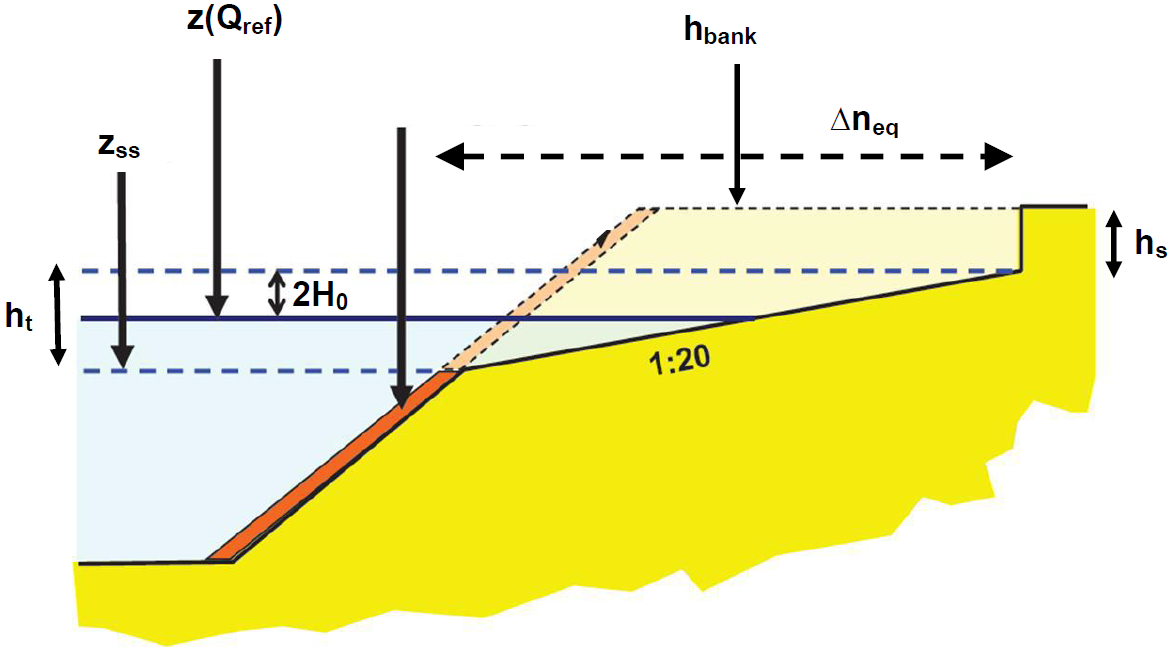
\includegraphics[width=\textwidth]{figures/Fig4-7.png}
\caption{Geschatte profiel evenwichtsoever.}
\label{Fig4.7}
\end{figure}

\section{Limitations of D-FAST Bank Erosion} \label{Sec4.7}

De oevererosiemodule is bedoeld als hulpmiddel om in te kunnen schatten waar potentieel oevererosie plaats kan vinden en niet om de daadwerkelijke oevererosie te voorspellen.
In deze sectie worden een paar beperkingen van de oevererosiemodule aangestipt.

\subsection{Homogeneous bank}

Een van de belangrijkste beperkingen is dat de samenstelling van de oever homogeen wordt verondersteld.
Dit is in de werkelijkheid niet het geval.
Er worden vaak horizontale of verticale lagen waargenomen.
In \autoref{Fig4.8} worden beide situaties weergegeven en de manier waarop het erosieproces plaatsvindt in het geval van horizontale lagen.
Om verticale lagen te kunnen modelleren, kunnen verschillende waarden van $c_E$ worden gebruikt voor elke laag.
De situatie met horizontale lagen is complexer, omdat in dit geval plotseling grote hoeveelheden oevermateriaal in een keer naar beneden kunnen glijden.

\begin{figure}
\begin{tabular}{p{6cm}p{6cm}}
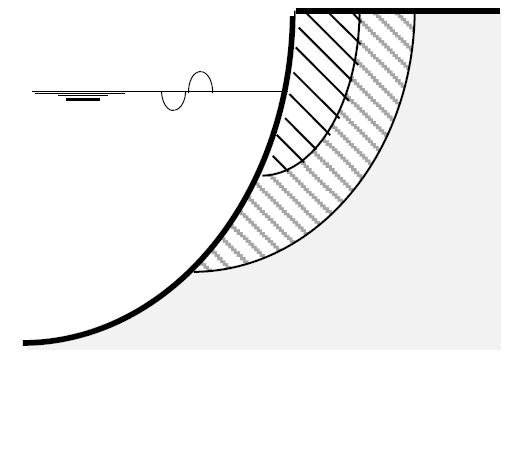
\includegraphics[width=5cm]{figures/Fig4-8a.png} \linebreak
a) vertical layers &
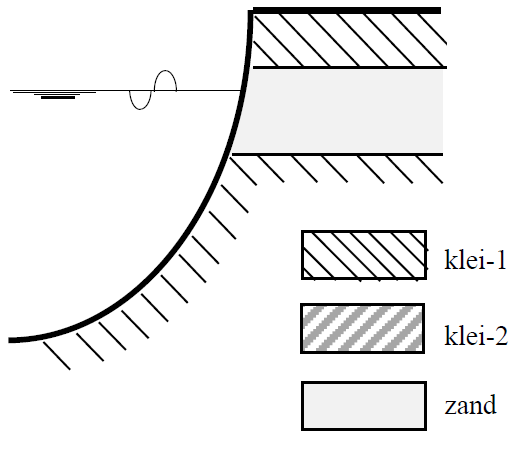
\includegraphics[width=5cm]{figures/Fig4-8b.png} \linebreak
b) horizontal layers \\
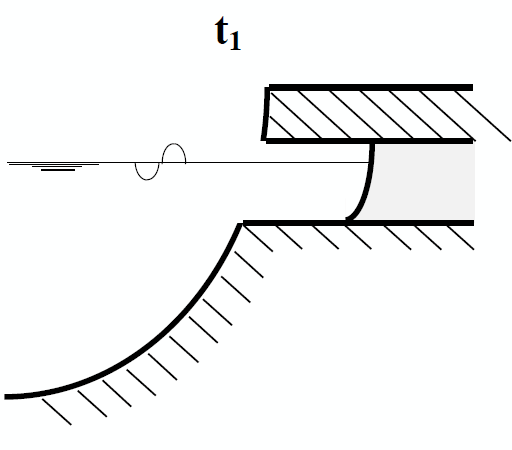
\includegraphics[width=5cm]{figures/Fig4-8c.png} \linebreak
c) erosion process in case of horizontal layers &
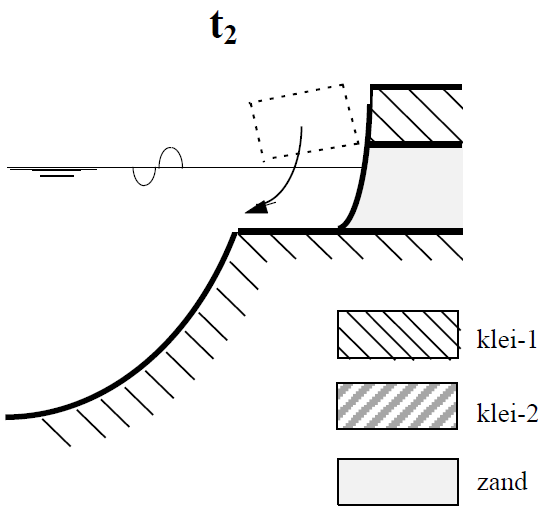
\includegraphics[width=5cm]{figures/Fig4-8d.png} \\
\end{tabular}
\caption{Non-homogeneous banks.}
\label{Fig4.8}
\end{figure}

\subsection{Only erosion along initial bank line}

Er wordt alleen oevererosie bepaald voor de opgegeven initiele oeverlijn (behorende bij een gemiddelde afvoer).
In werkelijkheid is het echter ook mogelijk dat er oevererosie op andere locaties plaatsvindt.

\subsection{Only erosion by ship waves and currents}

In de oevererosiemodule wordt alleen erosie door scheepsgolven en stroming gemodelleerd.
Andere erosiemechanismen zoals windgolven, uitstromend grondwater, bevriezing en vertrapping door vee worden in de module niet meegenomen.

\subsection{Profile and bed level remain constant}

Door oevererosie verandert lokaal de breedte van de rivier en ook zorgt het afgeslagen materiaal voor een andere bodemligging.
Hierdoor veranderen ook de stromingscondities in de rivier en langs de oever.
Aangezien de oevererosiemodule is gebaseerd uitkomsten van D-Flow FM berekeningen wordt deze dynamiek van de bodem en oevers echter niet meegenomen.


\nonumchapter{References}
Crosato, A. (2007), Effects of smoothing and regridding in numerical meander migration models. Water Resources Research, Vol 43.

CUR, (1996). Erosie van onverdedigde oevers, CUR-rapport 96-7, Gouda.

IWACO, Waterloopkundig Laboratorium en CSO (1998). Trajectnota/MER Zandmaas-Maasroute, Ontwerp natuurvriendelijke oevers. eindrapport 3361070.

Mark, R. van der, R.A.M. van der Sligte, A. Becker, E. Mosselman \& H.J. Verheij (2011), Morfologische effectstudie KRW-maatregelen IJssel.
Rapport 1204885, Deltares, Delft.

Schuurman, F. (2010), Casestudie oevererosie Maas, DHV memo kenmerk LW-AF20100800/RK, 30 december 2010.

Sieben, J., J.A.F. van Essen, M.J.M. Scholten and L.W.J. van Hal, (2005), Inschatting van de kans op achterloopsheid bij kribben, RIZA werkdocument 2005.148x.

Sieben, J. (2005), Wie het water deert, die het water keert - Inventarisatie van beheer en onderhoud van kribben en oeververdedigingen, RIZA werkdocument 2005.034x.

Spruyt, A. (2009), Shifting margins, behaviour of dynamic banks, Internal memorandum 200186-003-ZWS-0003-v2-m-Oeverdetectie, Deltares, Delft, 4 november 2010.

Spruyt, A. \& E. Mosselman (2010), Deelproject 3: Schuivende marges, gedrag van dynamische oevers (Shifting margins, behaviour of dynamic banks).
Appendix C in TO Rivierkundige Onderzoeksthema's; Rapportage 2009, Rapport 1200186.000, Deltares.

Stolker, C. \& H.J. Verheij (2001a), Gevoeligheidsonderzoek sedimentatie en erosie in kribvakken langs de Lek. Rapport Q2792, WL | Delft Hydraulics, Delft, Februari 2001.

Stolker, C. \& H.J. Verheij (2001b), Calibratie van een oeverafslagmodel voor de Zandmaas. Rapport Q3060, WL | Delft Hydraulics, Delft, November 2001.

TAW (1998), Technisch rapport erosiebestendigheid van grasland als dijkbekleding, Technische Adviescommissie voor de Waterkeringen, Delft.

Verheij, H.J., Meijer, D.G., Kruse, G.A.M., Smith, G.M., Vesseur, M., (1995). Investigation of the strength of a grass cover upon river dikes [in Dutch], Report Q1878, Deltares, Delft.

Verheij, H.J. (2000), Samenwerkingsproject Modellering Afslagoevers. Rapport Q2529, WL | Delft Hydraulics, Delft.

Verheij, H.J., F. van der Knaap \& H. Sessink (2007), Verder ontwikkelen van oeverafslagmodel BEM. Rapport Q4264.02, WL | Delft Hydraulics, Delft.

Vroeg, J.H. de (1999), Breach growth in cohesive materials : selection of cases. Rapport H3468, WL | Delft Hydraulics, Delft.

%\bibliography{../common/deltares_manual}

\appendix
\chapter{Bank strength coefficients for different soil types} \label{bankcomp}

The strength coefficient of the bank material, $c_E$ , and the critical shear stress for erosion, $\tau_c$, for different soil types are given in \autoref{Tab5.1} based on \citep{VerheijMKSV95, Vergeer96, VerheijKNS98, Vroeg99}.

The following relation can be used

\begin{equation}
c_E = \frac{\beta}{\tau_c}
\end{equation}

where $\beta$ = $1.85 \cdot 10^{-4}$ \unitbrackets{kg / (m\textsuperscript{2} s\textsuperscript{3})}.

\begin{table}[H]
\center
\begin{tabular}{p{5cm}rr}
Bank type & $c_E$ \unitbrackets{m\textsuperscript{-1}s\textsuperscript{-1}} & $\tau_c$ \unitbrackets{Pa} \\ \hline
Protected bank & 0 & $\infty$ \\
Sturdy grass & 0,01 $10^{-4}$ & 185 \\
Mediocre grass & 0,02 $10^{-4}$ & 93 \\
Bad grass & 0,03 $10^{-4}$ & 62 \\
Very good clay (compact) & 0,5 $10^{-4}$ & 4 \\
Clay with 60\% sand (firm) & 0,6 $10^{-4}$ & 2,5 \\
Good clay with  little structure & 0,75 $10^{-4}$ & 2 \\
Strongly structure good clay (mediocre) & 1,5 $10^{-4}$ & 1,5 \\
Bad clay (weak) & 3,5 $10^{-4}$ & 0,65 \\
Sand with 17\% silt & 10 $10^{-4}$ & 0,20 \\
Sand with 10\% silt & 12,5 $10^{-4}$ & 0,15 \\
Sand with 0\% silt & 15 $10^{-4}$ & 0,10 \\ \hline
\end{tabular}
\caption{Corresponding values for $c_E$ and $\tau_c$ \citep{VerheijMKSV95}.}
\label{Tab5.1}
\end{table}

\chapter{Determining ship induced wave height at the beginning of the fore shore} \label{Chp:shipwaves}

To determine the ship induced wave height $H_0$ \unitbrackets{m} at the beginning of the fore shore, the following formula is used (source: Handleiding DIPRO, 1997)

\begin{equation}
H_0 = \alpha_1 h \left ( \frac{s}{h} \right )^{-1/3} Fr^4
\end{equation}

with

\begin{symbollist}
\item[$\alpha_1$] ship dependent coefficient \unitbrackets{-}
\item[$Fr$] Froude number ($Fr$<0.8) \unitbrackets{-}
\item[$h$] water depth (considering a  trapezoidal profile) \unitbrackets{m}
\item[$s$] distance of shore to ship \unitbrackets{m}
\end{symbollist}

The Froude number is computed according to:

\begin{equation}
Fr = \frac{v_s}{\sqrt{g h}}
\end{equation}

with

\begin{symbollist}
\item[$g$] gravity acceleration 9.81 \unitbrackets{m/s\textsuperscript{2}}
\item[$v_s$] ship velocity \unitbrackets{m/s}
\end{symbollist}

The value of the Froude number is limited to 0.8.

For the coefficient $\alpha_1$ the following values are used, with $T_s$ \unitbrackets{m} the draught of the ships:

\begin{tabular}{ll}
Ship type & $\alpha_1$ \\ \hline
Push barge & 0.5 \\
RHK ship / Motorship & 0.28 $T_s^\text{1.25}$ \\
Towboat & 1.0 \\ \hline
\end{tabular}

By using this formulas, the value of $H_0$ can be computed based on the dominant ship type, their velocity and draught, the distance between fairway and shore and the water depth.

To prevent wave load on smaller channels far from the main channel, the wave height is smoothly reduced to zero from distance $s_1$ to $s_0$ from the fairway.
This is accomplished by multiplying $H_0$ with the following function:

\begin{equation}
f(s) = \left \{ \begin{matrix}
1 & 0 < s < s_1 \\
\cos \left ( \frac{s - s_1}{s_0 - s_1} \pi \right ) & s_1 < s < s_0 \\
0 & s > s_0
\end{matrix} \right .
\end{equation}

The value for $s_0$ will be in the order of 150 - 200 m and for  the following relation is used: $s_1 = s_0 - 50$.
In \autoref{Fig5.1} the wave height $H_0$ as function of the distance from the fairway $s$ is depicted for various values of the water depth $h$ for a moter ship with a draught of 1.2 m with a relative velocity of $v_s = 6$ m/s.
The wave height is reduced to zero between $s_1 = 100$ m and $s_0 = 150$ m.

\begin{figure}
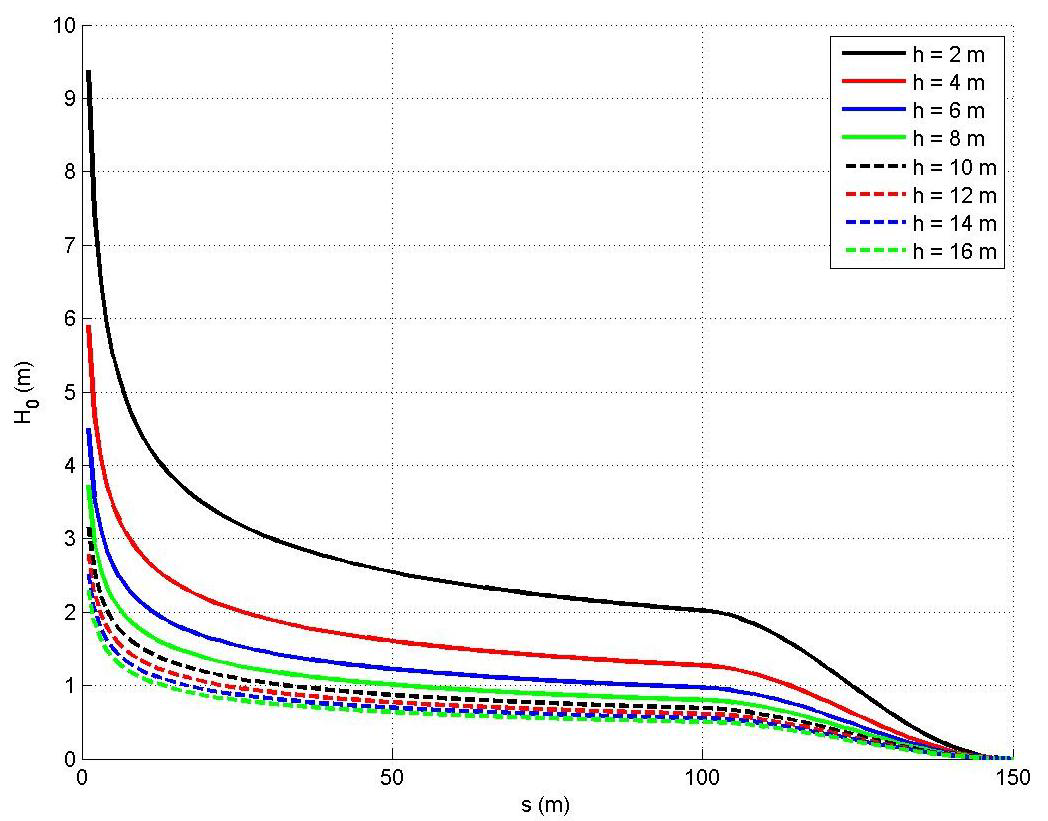
\includegraphics[width=\textwidth]{figures/Fig5-1.png}
\caption{Wave height as function from the distance from the fairway for different values of the water depth.}
\label{Fig5.1}
\end{figure}

\markdownInput{techref.md}

\pagestyle{empty}
\cleardoublepage
\mbox{}
\includepdf[pages=2, offset=-72 -70]{cover/d-fast-bank-erosion.pdf} % links-rechts past precies
\end{document}
